%Dokumentklasse
\documentclass[a4paper,12pt]{scrreprt}
\usepackage[left= 2.5cm,right = 2cm, bottom = 4 cm]{geometry}
%\usepackage[onehalfspacing]{setspace}
% ============= Packages =============


% Dokumentinformationen
\usepackage[
	pdftitle={Bachelorarbeit},
	pdfsubject={},
	pdfauthor={Santoro Sandro, Brunner Gian},
	pdfkeywords={},	
	%Links nicht einrahmen
	hidelinks]{hyperref}

% Standard Packages
\usepackage[utf8]{inputenc}
\usepackage[ngerman]{babel}
\usepackage[T1]{fontenc}
\usepackage{graphicx}
\graphicspath{{img/}}
\usepackage{lmodern}
\usepackage{color}
\usepackage{siunitx}
\usepackage{tikz}
\usepackage{caption}
\usepackage{placeins}
\usepackage{tabularx}
\usepackage{arydshln}
\usepackage{pdfpages}
\usepackage{listings}
\usepackage{url}
\usepackage{mathtools}
\usepackage{makecell}
\usepackage{multirow}
\usepackage{booktabs}
\usepackage{float}
\usepackage{apacite}

\sisetup{detect-weight=true, detect-family=true}
\newcommand{\source}[1]{\caption*{Source: {#1}} }


% ============= Kopf- und Fußzeile =============

\usepackage[automark,headsepline]{scrlayer-scrpage} %footsepline
\pagestyle{scrheadings}
\automark[chapter]{chapter}
\clearscrheadfoot

\ihead{\headmark}				%Kopfzeile innen mit Kapitel
\chead{}						%Kopfzeile Mitte
\ohead[\pagemark]{\pagemark}	%Kopfzeile aussen mit Seitennummer

%\ifoot{}						%Fußzeile innen
%\cfoot{}						%Fußzeile Mitte
%\ofoot{}						%Fußzeile außen

\renewcommand*\chapterpagestyle{scrheadings}

%============== Abstände von Kopfzeile zu Text überall gleich ============%
\renewcommand*\chapterheadstartvskip{\vspace*{-\topskip}}
\renewcommand*\chapterheadendvskip{%
\vspace*{1\baselineskip plus .1\baselineskip minus .167\baselineskip}}


% zusätzliche Schriftzeichen der American Mathematical Society
\usepackage{amsfonts}
\usepackage{amsmath}
\usepackage{cleveref}

%nicht einrücken nach Absatz
\setlength{\parindent}{0pt}

%============== Package für Dateistruktur-Baum ============%
\usepackage{forest}

% ============= Package Einstellungen & Sonstiges ============= 
%Besondere Trennungen
\hyphenation{De-zi-mal-tren-nung}


%=========== Abbildungen fangen mit 1 an ===========%
\renewcommand*{\thefigure}{\arabic{figure}}


% ============= Dokumentbeginn =============
\begin{document}
\setcounter{secnumdepth}{4}	%Bis wo das nummeriert wird (4te Ebene)
\setcounter{tocdepth}{4}

%Seite ohne Kopf- und Fußzeile sowie Seitenzahl
\thispagestyle{empty}

\renewcommand*\chapterpagestyle{scrheadings}

\includegraphics[scale=0.5]{img/ntb.jpg}

\begin{center}
\vspace*{4 cm}
\textbf{\Huge Bachelorarbeit}
\end{center}

\begin{center}
\vspace*{1.5 cm}
\LARGE{\textsf{Menü-Crawler\\}}
\large{\textsf{Prototyp einer Search Engine zur Suche von Speisen und Menüs in der deutschsprachigen Schweiz\\}}
\end{center}


\begin{center}
\vspace*{2 cm}
\textbf{ Studierende:} {\textbf{Sandro Santoro \& Gian Brunner\\}}
\end{center}

\begin{center}
\vspace*{1 cm}
Abgabedatum: 9. August 2019
\vspace*{1 cm}
\end{center}


\begin{center}
\begin{tabular}{lll}
\textbf{Referent:} & & Prof. Corsin Capol\\
\medskip
\textbf{Korreferent:} & & Lukas Toggenburger\\
\end{tabular}
\end{center}


\pagestyle{scrheadings}
\pagenumbering{Roman}

\addchap{Abstract}
\addsec{Abstract Deutsch}
Die Idee dieser Arbeit ist das Erstellen einer Suchmaschine, über welche sich Restaurant-übergreifend Menüs und Speisen suchen lassen.
Die Grundlage einer solchen Suchmaschine sind die Websites von Restaurants in Kombination mit Informationen wie z.B. dem Standort.
Um einen Datensatz solcher Websites zu erstellen, ist ein Webcrawler implementiert worden.
Im wissenschaftlichen Teil dieser Arbeit wurde anhand dieses Datensatzes ein Gold Standard erstellt.
Dieser dient dazu, die eigentliche Forschungsfrage beantworten zu können, die folgendermassen lautet:\\
\emph{Können Restaurant-Webseiten mit hoher Wahrscheinlichkeit klassifiziert werden, ob sie Menüinformationen beinhalten?}\\
Vorausgesetzt wird ein F1-Score von 0.8 oder höher, um diese Frage mit \glqq Ja\grqq{} beantworten zu können.
Dabei werden zwei verschiedene Ansätze zur Klassifikation angewandt, namentlich das regelbasierte Klassifizieren sowie das Klassifizieren mittels Machine-Learning.
Um diese Ansätze prüfen zu können, werden mehrere Experimente durchgeführt.
Zum Schluss wird erkannt, dass der gewünschte F1-Score mit beiden Ansätzen knapp verfehlt wurde.
Im praktischen Teil wird neben dem Webcrawler eine Webapplikation erarbeitet, welche als Suchmaschine dient und die klassifizierten Daten dem Benutzer darstellt.
\addsec{Abstract English}
The idea of this work is to create a search engine that can be used to search menus and meals restaurant independently.
The basis of such a search engine are the websites of restaurants in combination with information such as, for example, the location.
To create a dataset of such websites, a web crawler has been implemented.
In the scientific part of this work, a gold standard was created based on this dataset.
This serves to answer the actual research question, which is the following: \\
\emph{Can Webpages of restaurants be classified with high chance of success, if they contain menu information?} \\
An F1 score of 0.8 or higher is required to answer this question with \glqq Yes\grqq{}.
Two different approaches are used for classification, in particular rule-based classification and classification with machine learning.
To be able to test these approaches, several experiments are carried out.
Finally, it is recognized that the desired F1 score was missed with both approaches.
In the practical part, in addition to the webcrawler, a web application will be developed which serves as a search engine and displays the classified data to a user.

\addchap{Danksagung}
Wir bedanken uns herzlich bei unseren Referenten, Corsin Capol und Lukas Toggenburger, dafür, dass sie uns bei dieser Arbeit viele Freiheiten gelassen und uns viele gute Ratschläge gegeben haben.\\
Zudem bedanken wir uns bei Norman Süsstrunk für die Hilfe bei der Erarbeitung des Webcrawlers.
\newpage

%Inhaltsverzeichnis
\tableofcontents

\clearpage 
\newpage

\addchap{Glossar}
Crawlen - Die Tätigkeit eines Webcrawlers: Das Aufrufen und Herunterladen von Webseiten\\
OSM - Opensteetmap, eine freie Geodatenbank\\
SDK - Software Development Kit (SDK) Programmierwerkzeug und Bibliothek, welches hilft, eine Software zu entwickeln\\
Seed - Eine Liste bestehend aus Webseiten, welche gecrawlt werden sollen\\
Stormcrawler - SDK zur Entwicklung eines Webcrawlers\\
Webcrawler - Programm zum automatisierten Aufrufen und Speichern einer Webseite\\
Website - Komplette Internetseite (Startseite inkl. allen Subwebsites) z.B. www.menucrawler.ch\\
Webpage - Spezifischer Teil einer Webseite z.B. www.menucrawler.ch/ueber-uns\\
idempotent - Bei gleicher Eingabe erfolgt stets die gleiche Ausgabe, egal wie oft die Aufgabe ausgeführt wird\\
Open-Source - Software, deren Quelltext frei einsehbar und änderbar ist\\
Big Data - Arbeitsumfeld, indem mit sehr vielen Datenpunkten gearbeitet wird\\
Machine-Learning - Maschinelles Lernen, der Computer wird darauf trainiert, eine Aufgabe zu verrichten\\
Pipelining - Das verbinden von mehreren Aufgaben zu einer Gesamtaufgabe\\
Stream - Kontinuierlicher Fluss von Datensätzen\\
URL - Uniform Ressource Locator - Eindeutiger Link zu einer Webpage\\
Blacklisting - Index, der zur Benachteiligung der darin aufgeführten Einträgen führt\\
Whitelisting - Index, der zur Bevorzugung der darin aufgeführten Einträgen führt\\
Labeling - Kategorisieren von Daten\\
JSON - JavaScript Object Notation, ein kompaktes Dateiformat in lesbarer Textform, geeignet für den Datenaustausch zwischen Anwendungen\\
No free lunch - Ein Theorem, welches besagt, dass es kein universelles Verfahren für die Lösung eines ML-Problems gibt\\
N-Gramme - Wörterkette mit Anzahl N Wörtern\\
Features - Merkmale, mit denen ein ML-Algorithmus trainiert werden kann\\
Feature-Extraction - Das Extrahieren von relevanten Features\\
LSA (Latent Sentiment Analysis) - Verfahren zum Auffinden von Schlüsselbegriffen\\
Bigramm - Eine Wörterkette mit Länge zwei\\
Trigramm - Eine Wörterkette mit Länge drei\\
Scores - Die Resultate, in diesem Zusammenhang die Resultate der Klassifizierer\\
API - Application Programming Interface (Applikationsprogrammierschnittstelle)\\
Data Mining - Behandlung von grossen Datenmengen um Zusammenhänge zu finden (z.B. Kaufverhalten von Nutzern anhand von Suchverläufen herausfinden)\\
BSD - Berkeley Software Distribution, eine Softwarelizenz, welche die Weiterbearbeitung von Quelltext erlaubt\\
Supervised Learning - Das maschinelle Lernen mit Daten, welche im Vorraus markiert worden sind (z.B. manuelles Markieren von Spam bei Emails)\\
Unsupervised Learning - Das maschinelle Lernen mit Daten, welche nicht markiert sind. Dadurch kann der Computer keine konkrete Klassifizierung machen, sondern nur Ähnlichkeiten in den Daten aufzeigen\\
Fast Prototyping - Das schnelle Entwickeln eines Prototypen, welche die Grundfunktionen mehr oder weniger befriedigend ausführt\\
NLP - Natural Language Processing, Verarbeitung natürlicher Sprache\\
Geolocation - Geografische Koordinaten eines Objekts

\newpage


\numberwithin{figure}{chapter}
\pagestyle{scrheadings}
\pagenumbering{arabic}

\chapter{Einleitung}
Viele Menschen nutzen das Internet, um sich über Speisekarten und Mittagsmenüs zu informieren.
Jedoch gibt es zur Zeit keine Suchmaschine, über welche sich Restaurant-übergreifend Speisen sowie Menüs suchen und finden lässt.
Diese Arbeit hat das Ziel, den Prototypen einer solchen Suchmaschine zu entwickeln.\\
Dazu werden verschiedene Teilkomponenten entwickelt, welche zusammen dieses Ziel erfüllen.
Bei der ersten Komponente handelt es sich um einen Webcrawler, welcher Websites automatisiert aufruft und speichert.
Jede Webpage dieser Websites wird dann mittels einer weiteren Komponente, dem Classifier, klassifiziert, ob es sich dabei um eine Menüseite oder Speisekarte handelt.
Webpages, welche als Menüseite oder Speisekarte klassifiziert wurden, werden in einer Search Engine gespeichert und verwaltet.
Als letzte Komponente kommt eine Webapplikation zum Einsatz. Ein Benutzer kann 
auf dieser Webapplikation nach einer Speise suchen und diese Suche optional 
mittels Standortfilter eingrenzen.\\
Diese Arbeit beinhaltet zwei verschiedene Teile, einen wissenschaftlichen und einen praktischen Teil.
Im wissenschaftlichen Teil wird die Klassifikation von Webpages methodisch erarbeitet.
Im praktischen Teil werden die klassifizierten Webpages über eine 
Webapplikation verfügbar gemacht.
\newpage

\chapter{Stand der Forschung}
\section{Gold Standard}
% Was definiert einen guten Gold Standard?
Öffentliche Datensätze, welche Daten in Textform beinhalten, sind in verschiedenen Kategorien verfügbar\footnote{\url{https://medium.com/@dataturks/rare-text-classification-open-datasets-9d340c8c508e} abgerufen am: 25.06.2019}.
Auch Datensätze, die Informationen über Menüs beinhalten, sind bereits öffentlich verfügbar\footnote{\url{https://data.world/data-society/discover-the-menu} abgerufen am: 25.06.2019}.
Deutsche Textdatensätze sind bereits weniger verbreitet wie solche in englischer Sprache\footnote{\url{http://wortschatz.uni-leipzig.de/en/download/} abgerufen am: 25.06.2019}.
Einen auf der deutschen Sprache basierender Datensatz, welcher Informationen über Menüseiten beinhaltet, konnte nicht gefunden werden.
\section{Klassifikation}
Eine Methode, um Text in verschiedene Kategorien zu klassifizieren, ist das Erstellen von Regeln.
Mit einem ausgefeilten Regelsatz kann dies bei einer geringen Anzahl verschiedener Kategorien gut funktionieren.
Das Erstellen eines solchen Regelsatzes ist zeitaufwendig und muss mit einem repräsentativen Datensatz überprüft werden.
Somit ist es ein iterativer Prozess und der Ersteller muss über Expertenwissen im Themengebiet verfügen.
Solche Regelsätze bestehen aus \glqq Wenn-Dann\grqq-Bedingungen, welche mit logischen \glqq UND\grqq{} bzw. \glqq ODER\grqq{} Operatoren verknüpft sind in Kombination mit regulären Ausdrücken.
Mit solchen Regelsätzen können hohe Scores erreicht werden, ein grosses Problem des Erstellens solcher Regelsätze ist jedoch der Zeitaufwand, denn dieser steigt linear mit der Komplexität.
Aus diesem Grund besteht ein hoher Bedarf, Daten mittels statistischer Methoden automatisiert zu klassifizieren, ohne dass ein Mensch zuerst neue Regelsätze implementieren muss.\\
An diesem Punkt kommen Machine-Learning-Algorithmen zum Zug.
Diese analysieren einen Datensatz, bei dem die Proben bereits eine Zuteilung zur jeweiligen Kategorie hinterlegt haben, und klassifiziert künftige Daten anhand dieser Analyse. \cite[p. 125-127]{jackson2007natural}
\section{No-Free-Lunch Theorem}\label{sec:nofreelunch}
Ein Theorem des bekannten Informatikers David H. Wolpert, welches sinngemäss die Aussage trifft, dass kein Klassifizierer existiert, welcher für eine Vielzahl von Klassifikationsproblemen geeignet wäre \cite[p. 1341-1390]{Wolpert1996TheLO}.
Wenngleich das No-Free-Lunch Theorem aus mathematischer Sicht korrekt ist, hat sich in der Praxis doch gezeigt, dass gewisse Klassifikation-Alogorithmen über mehrere Problemklassen hinweg gute Resultate erzielen \cite{fernandez-delgado2014}.
\section{Klassifikationsalgorithmen}\label{sec:algos}
\subsection{Lineare Modelle}
Lineare Modelle basieren auf der Annahme, dass ein linearer Zusammenhang zwischen Eingangsvariablen und Ausgangsvariablen besteht.
Sie versuchen Parameter zu einer linearen Gleichung zu finden, welche die Trainingsdatenpunkte optimal abdecken.
Das optimale Abdecken wird mit einer Loss-Funktion ermittelt.
Die Loss-Funktion berechnet den Unterschied zwischen vorhergesagtem Wert zu tatsächlichem Wert des Trainingsdatenpunktes.
Lineare Modelle verwenden Optimierungsverfahren, welche iterativ Parameter verändern, um die Werte der Loss-Funktion zu minimieren und somit die bestmögliche Parameterzusammensetzung zu ermitteln.\cite{Frick-Wuersch}
\subsubsection{Ridge Classifier}
Der Ridge Classifier ist ein linearer Klassifizierer, welcher als Loss-Funktion die \glqq Least Square\grqq{} Funktion (eine Minimierung der quadrierten Abweichungen) und als Regularisierung die L2-Norm verwendet. Die L2-Norm wird pythagoreisch aus den Vektorwerten berechnet\footnote{\url{https://machinelearningmastery.com/vector-norms-machine-learning/} abgerufen am: 13.07.2019}.
Die Kombination aus oben erwähnter Loss-Funktion und der L2-Norm wird auch \glqq Ridge Regression\grqq{} genannt, von welcher der Klassifizierer auch seine Bezeichnung erhielt\footnote{\url{https://scikit-learn.org/stable/modules/generated/sklearn.linear_model.Ridge.html} abgerufen am: 13.07.2019} \cite{scikit-learn}.
\subsubsection{PassiveAgressive Classifier}
Der PassiveAggressive Classifier ist ein Klassifizierer für grosse Datenmengen.
Er ist verwandt mit dem Perceptron Algorithmus, da er keine Lernrate benötigt.
Der Klassifizierer funktioniert grob umschrieben so, dass wenn die Klassifizierung korrekt ist, er sich passiv verhält und seine internen Gewichte nicht anpasst.
Erst bei einer falschen Klassifizierung änderen seine interne Gewichte aggressiv, so dass die Fehlklassifizierung behoben wird. \cite{crammer2006online}
\subsubsection{SGDClassifier}
Der SGDClassifier gehört zur Familie der linearen Modelle\footnote{\url{https://scikit-learn.org/stable/modules/generated/sklearn.linear_model.SGDClassifier.html} abgerufen am: 14.05.2019} \cite{scikit-learn}.\\
Der \glqq Stochastic-Gradient-Descent-Classifier\grqq{} verwendet als Optimierungsvefahren das \glqq Stochastic Gradient Descent\grqq{} Verfahren\footnote{\url{https://scikit-learn.org/stable/modules/sgd.html} abgerufen am: 14.05.2019}.
Bei diesem kommt der mathematische Gradient zum Einsatz.
Der Gradient zeigt bei der Optimierung der Parameter immer in die Richtung, in welcher der Fehler (gemessen an der Loss-Funktion) am stärksten minimiert werden kann.\\
Der stochastische/probabilistische Anteil dieses Verfahrens bedeutet, dass bei der Berechnung des Gradienten jeweils nur ein Subset des ganzen Trainingsdatensatzes verwendet wird.
Dies hat den Vorteil, dass die Trainingszeit optimiert werden kann und zugleich gute Werte erzielt werden können \cite{lecun2012efficient}.\\
In der \cref{fig:sgd} wird der Verlauf der Loss-Funktion aufgezeigt und wie der Gradient zu interpretieren ist.
\begin{figure}[H]
	\centering	
	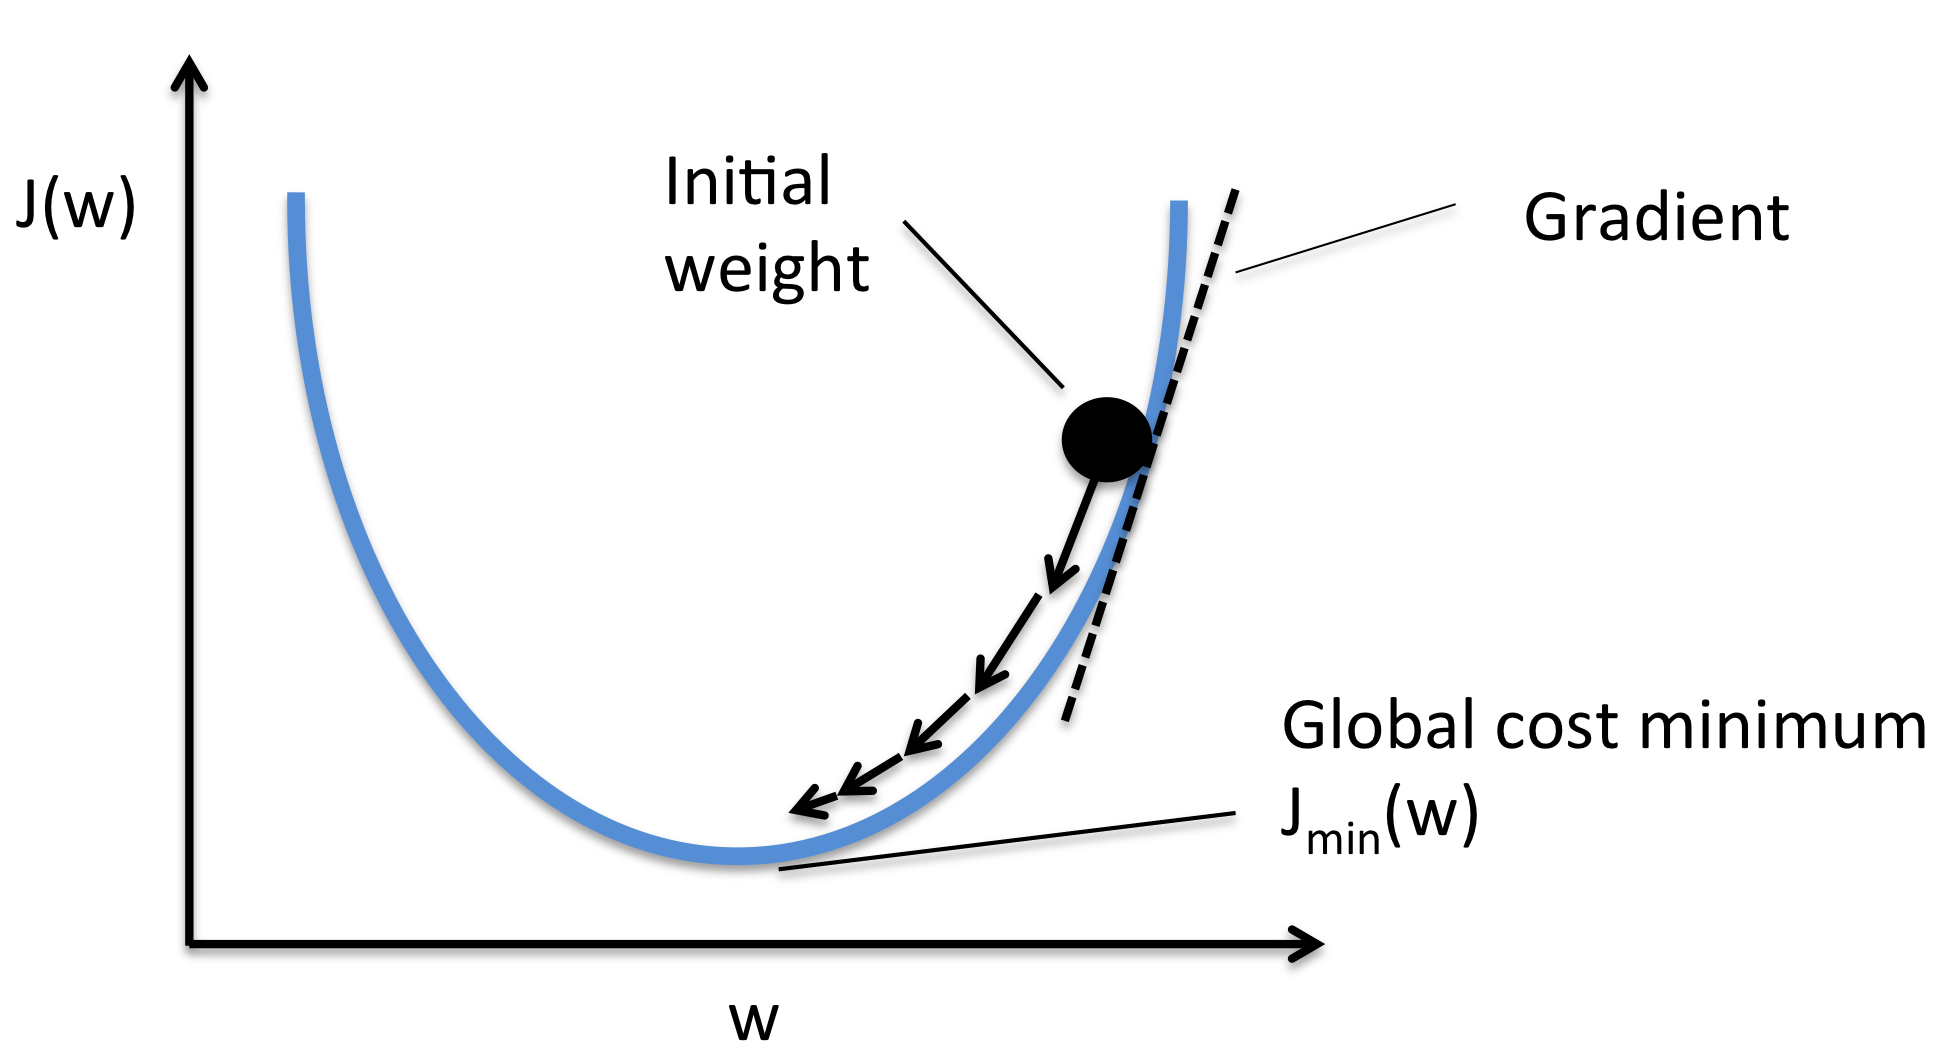
\includegraphics[width=0.7\columnwidth,keepaspectratio]{img/sgd.png}
	\caption{Visualisierung des Gradienten und der Loss-Funktion (J(w) = Loss; w = Parameteränderung)}
	\source{\url{http://rasbt.github.io/mlxtend/user_guide/general_concepts/gradient-optimization/} aufgerufen am: 05.08.2019}
	\label{fig:sgd}
\end{figure}
\subsubsection{Perceptron}
In der \cref{fig:perceptron-grafik} ist die Darstellung eines Perceptrons ersichtlich.
Ein Perceptron ist ein Knoten, welcher allen Input-Variablen \glqq x1-x3\grqq{} eine Gewichtung (Ein Mass für die Wichtigkeit) \glqq w1-w3\grqq{} zuweist.
Die gewichteten Inputs werden dann aufsummiert.
Wenn die Summe einen bestimmten Schwellwert überschreitet, schaltet der Ausgang \glqq y\grqq{} seinen Zustand um.\\
Ein einzelnes Perceptron kann als binärer Klassifizierer verwendet werden.
Im Deep-Learning Umfeld werden mehrere Perceptronen miteinander verbunden, um ein neuronales Netzwerk zu erstellen\footnote{\url{https://towardsdatascience.com/perceptron-the-artificial-neuron-4d8c70d5cc8d} abgerufen am: 05.08.2019}.
\begin{figure}[H]
	\centering	
	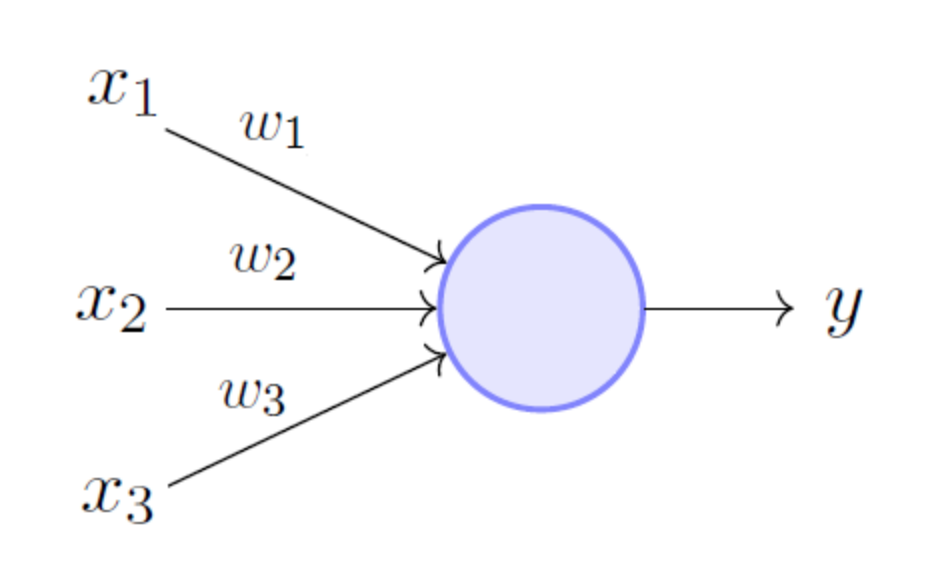
\includegraphics[width=0.6\columnwidth,keepaspectratio]{img/perceptron.png}
	\caption{Visualisierung eines Perceptrons}
	\source{\url{https://towardsdatascience.com/perceptron-the-artificial-neuron-4d8c70d5cc8d?} aufgerufen am: 05.08.2019}
	\label{fig:perceptron-grafik}
\end{figure}
\subsection{Naive Bayes}
Naive Bayes Algorithmen sind ein Set von Supervised Learning Algorithmen, welche auf dem Theorem von Bayes basieren.\\
Das Bayes Theorem zeigt die Berechnung von bedingten Wahrscheinlichkeiten auf:
$$ P(A \mid B) = \frac{P(B \mid A) \,* P(A)}{P(B)} $$
$$ P(A) = Wahrscheinlichkeit\ von\ Ereignis\ A$$
$$ P(B) = Wahrscheinlichkeit\ von\ Ereignis\ B$$
$$ P(A \mid B) = Wahrscheinlichkeit\ von\ Ereignis\ A\ nach\ eintreffen\ von\ Ereignis\ B$$
$$ P(B \mid A) = Wahrscheinlichkeit\ von\ Ereignis\ B\ nach\ eintreffen\ von\ Ereignis\ A$$
Das Bayes Theorem kann zur Hilfe genommen werden, um bedingte Ereignisse zu berechnen\footnote{\url{https://www.crashkurs-statistik.de/der-satz-von-bayes/} abgerufen am: 16.07.2019}.
Der naive Vorsatz deutet auf die Annahme des Theorems, dass eine vollständige Unabhängigkeit zwischen allen Features herrscht.
Diese Annahme ist in der realen Welt oft nicht korrekt, trotzdem können Naive Bayes Algorithmen gute Scores erreichen und werden oft als Referenz verwendet. \cite{rennie2003tackling}
\subsubsection{Multinomial Naive Bayes}
Der Multinomial Naive Bayes Algorithmus verwendet die Annahme, dass die unabhängigen Features einer Multinomialverteilung folgen.
Für jede Klasse werden Multinomial-Parameter bestimmt.
Diese Parameter sind Vektoren, welche die Wortwahrscheinlichkeiten, dass die Wörter in den entsprechenden Klassen vertreten sind, aufzeigen.
Die Wahrscheinlichkeit, dass ein Dokument zu einer Klasse gehört, wird mit dem Produkt aller Wortwahrscheinlichkeiten aus den Vektoren bestimmt, welche sich im Dokument befinden. \cite{rennie2003tackling}
\subsubsection{Gaussian Naive Bayes}
Der Gaussian Naive Bayes Algorithmus verwendet die Annahme, dass die unabhängigen Features einer Normalverteilung folgen\footnote{\url{https://scikit-learn.org/stable/modules/naive_bayes.html} abgerufen am: 16.07.2019} \cite{scikit-learn}.
\subsubsection{Bernoulli Naive Bayes}
Der Bernoulli Naive Bayes Algorithmus verwendet die Annahme, dass die unabhängigen Features einer Bernoulliverteilung folgen.
Die Features werden als binäre Vektoren dargestellt.
Somit wird nur das Vorhandensein und nicht die Häufigkeit der Features appliziert.
Ebenfalls werden alle Relationen zwischen den unterschiedlichen Features mit der strikten Einhaltung der binären Bernoulliverteilung entfernt. \cite{mccallum1998comparison}
\subsubsection{Complement Naive Bayes}
Der Complement Naive Bayes Algorithmus (CNB) ist eine Abwandlung des Multinomial Naive Bayes Algorithmus.
Er eignet sich für stark ungleiche Datensets und verwendet für das Setzen der internen Gewichte die Komplemente der einzelnen Klassen.
Das heisst, um die Gewichte für die Klasse A zu setzen, werden alle Klassen ausser A für die Berechnung der Gewichte verwendet. \cite{rennie2003tackling}
\subsection{DecisionTree}\label{sec:trees}
Der DecisionTree-Algorithmus baut schrittweise eine Baumstruktur von Entscheidungszweigen auf, um eine Klassifizierungsaufgabe zu meistern.
DecisionTrees versuchen eine komplexe Aufgabe in Teilprobleme zu zerlegen und diese mit einfachen Entscheidungen zu bewältigen.
DecisionTree-Strukturen können verbessert werden, indem die Tiefe der Äste oder die Anzahl der Äste angepasst wird.
Bei stetiger Erhöhung der Tiefe oder der Anzahl der Äste steigt auch die Zeitkomplexität der DecisionTrees. \cite{safavian1991survey}
\subsection{Ensemble-Learning}
Ensemble-Learning ist ein Zusammenschluss von mehreren unterschiedlichen Klassifizierern, welche mit einem Voting-Verfahren eine schlussendliche Klassifizierung durchführen.
Ensemble-Learning basiert auf der Annahme, dass mehrere Algorithmen im Plenum eine bessere Aussage liefern können als ein Algorithmus alleine. \cite{freund1999short}
\subsubsection{RandomForestClassifier}
RandomForest gehört ebenfalls zur Familie der Ensemble-Learner\footnote{\url{https://scikit-learn.org/stable/modules/generated/sklearn.ensemble.RandomForestClassifier.html} abgerufen am: 14.05.2019}.
RandomForest ist eine Zusammensetzung von mehreren unterschiedlichen DecisionTrees (siehe \cref{sec:trees}).\\
RandomForest verwendet nun eine Vielzahl von DecisionTrees, die alle unterschiedliche Tiefen oder Anzahl Äste besitzen.
Dadurch können Entscheidungsausreisser aufgefangen und durch den Mehrheitsentscheid gedämpft werden. \cite{liaw2002classification}
\subsubsection{AdaBoostClassifier}
Bei vielen Ensemble-Verfahren werden alle Klassifizierer parallel trainiert und geben ihr Votum gleichzeitig ab.
Adaboost verwendet jedoch die Methode des \glqq Boosting\grqq{}, welche Ähnlichkeit mit der Theorie der genetischen Algorithmen hat\footnote{\url{https://scikit-learn.org/stable/modules/ensemble.html} abgerufen am: 14.05.2019}.
Bei Adaboost wird ein Algorithmus trainiert, validiert und als Ursprung verwendet. Alle zusätzlichen Algorithmen, welche das finale Voting durchführen, werden vom Ursprungsalgorithmus abgeleitet.
Es werden jedoch bei den Abkömmlingen die internen Parameter schrittweise verbessert und versucht die Fehler des \glqq Vater-Algorithmus\grqq{} zu vermeiden.
AdaBoost kann verbessert werden, indem die Anzahl von Vererbungsschritten angepasst wird. \cite{freund1999short}
\subsection{Nearest Neighbor Modelle}
Der Nearest Neigbhor (NN) Algorithmus ist einer der simpelsten Entscheidungsprozesse für Klassifikationen.
Beim NN Algorithmus werden Datenpunkte entsprechend ihren nächsten Nachbarn klassifiziert. \cite{cover1967nearest}
Dieses Verhalten ist in der \cref{fig:knn} für unterschiedliche Schwellwerte der Anzahl Nachbarn ersichtlich.
\begin{figure}[H]
	\centering	
	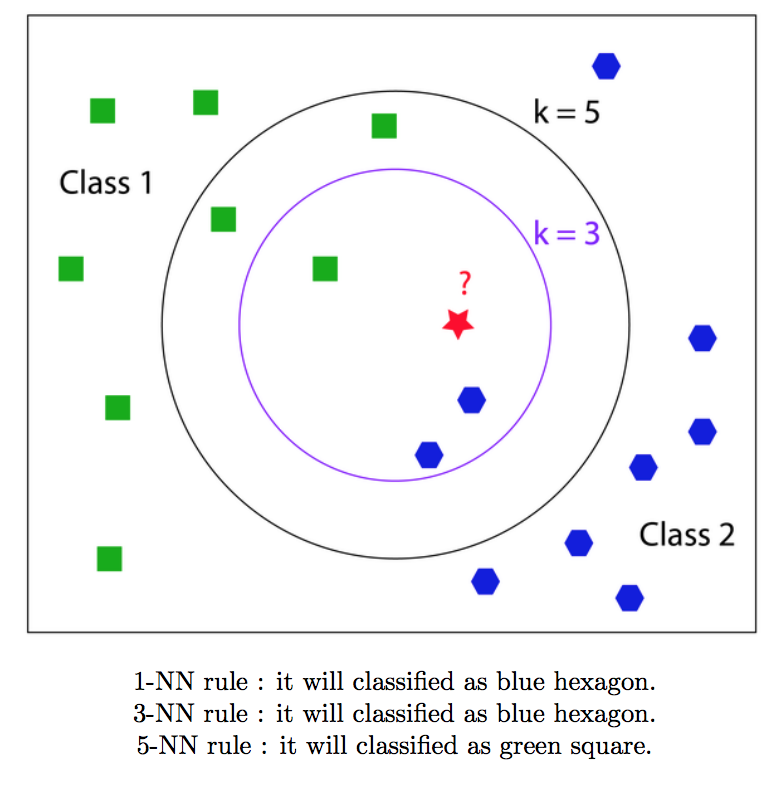
\includegraphics[width=0.7\columnwidth,keepaspectratio]{img/knn.png}
	\caption{Darstellung einer simplen K-Nearest Neighbor Prozedur}
	\source{\cite{cover1967nearest}}
	\label{fig:knn}
\end{figure}
\subsubsection{K-Nearest-Neighbor}
Der KNN Algorithmus funktioniert nach dem gleichen Prinzip wie der NN Algorithmus.
Ein Unterschied ist, dass eine spezifische Anzahl von Nachbarn mit der Kennzahl K definiert wird.
Alle K-nächsten Datenpunkten klassifizieren den gesuchten Datenpunkt mit einem Mehrheitsentscheid.
Dies ist in der \cref{fig:knn} für K=3 und K=5 ersichtlich.
K kann frei gewählt werden und dient hervorragend als Parameter für ein Hyperparametertuning (siehe \cref{sec:hyp}). \cite{cover1967nearest}
\subsubsection{Nearest Centroid}
Der Nearest Centroid Algorithmus basiert auf dem Prinzip des NN Algorithmus.
Zuerst werden die Schwerpunkte aller Klassen berechnet, indem alle zur Klasse zugewiesenen Datenpunkte miteinbezogen werden.
Danach wird der zu klassifizierende Datenpunkt der Klasse mit der kleinsten Differenz von Datenpunkt zu Schwerpunkt der Klasse zugewiesen.
Somit wird für den Nearest Centroid Algorithmus nicht der Mehrheitsentscheid der nächsten Nachbarn zur Klassifikation verwendet, sondern die Distanzen zu den Klassenschwerpunkten\footnote{\url{https://scikit-learn.org/stable/modules/neighbors.html} abgerufen am: 14.05.2019}. \cite{scikit-learn}
Dieses Verhalten ist in \cref{fig:centroid} ersichtlich.
Die schwarzen Datenpunkte markieren jeweils den Schwerpunkt der entsprechenden Klasse und die Abgrenzung der einzelnen Klassen ist mit gestrichenen, schwarzen Linien dargestellt.
\begin{figure}[H]
	\centering	
	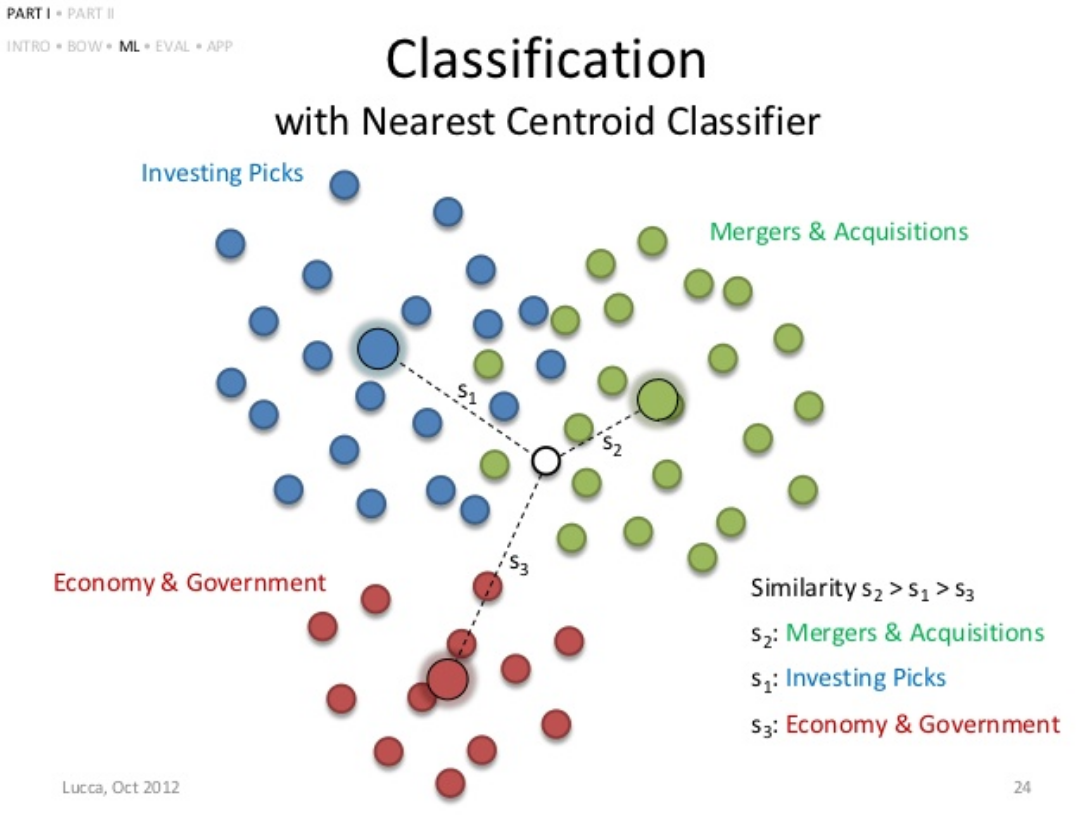
\includegraphics[width=0.7\columnwidth,keepaspectratio]{img/centroid.png}
	\caption{Darstellung einer simplen Nearest Centroid Prozedur}
	\source{\url{https://www.researchgate.net/figure/Abbildung-410-Illustration-des-Nearest-Centroid-Verfahrens-mit-den-Gruppen-soft_fig4_267488030} aufgerufen am: 14.05.2019}
	\label{fig:centroid}
\end{figure}
\subsection{Support Vector Machine Modelle}
SVM-Classifier (Support Vector Machine) erzielen gute Resultate bei der Klassifizierung von Textdateien.
Ein Vorteil von SVM ist, dass ihre Lernrate unabhängig von der Dimension der Features ist. \cite{joachims1998text}
Dies wird erreicht, da SVM nicht auf die ganzen Features angewiesen ist.
Zwischen den unterschiedlichen Klassen werden Hyperebenen gelegt, welche das Ziel haben, die Abstände zu den einzelnen Klassen zu maximieren.
In der \cref{fig:svm} ist eine solche Hyperebene ersichtlich.
Die Features, welche am nächsten zu den Hyperebenen liegen, werden Support Vektoren genannt.
Der Algorithmus kann nach der Trennung der Klassen nun die Position von neuen Features bestimmen und somit eine Schätzung einer geeigneten Klasse vornehmen. \cite{tong2001support}
\begin{figure}[H]
	\centering	
	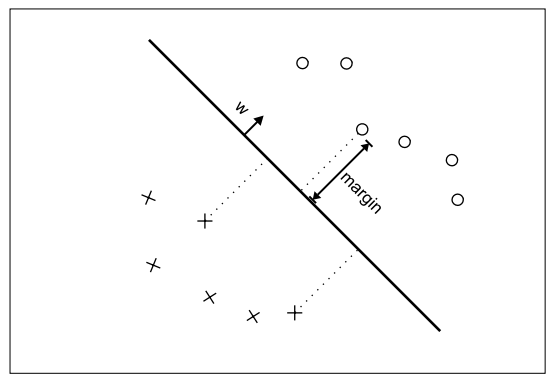
\includegraphics[width=0.7\columnwidth,keepaspectratio]{img/svm.png}
	\caption{Darstellung einer simplen Support Vector Machine}
	\source{\cite{tong2001support}}
	\label{fig:svm}
\end{figure}
\section{Hyperparametertuning}\label{sec:hyp}
Parameter, welche nicht selbstständig vom Machine-Learning Modell angepasst werden können, werden Hyperparameter genannt.
Diese Hyperparameter definieren das Verhalten von den Modellen.
Die geeignetsten Hyperparameter können mit einer ausführlichen Suche gefunden werden, was als Hyperparametertuning bezeichnet wird\footnote{\url{https://scikit-learn.org/stable/modules/grid_search.html} abgerufen am: 14.05.2019}. \cite{scikit-learn}
\newpage

\chapter{Methodik}
\section{Forschungsfrage}
Die Forschungsfrage, welcher mit dieser Arbeit beantwortet wird, lautet wie folgt:\\
\emph{Können Webpages von Restaurant-Websites mit hoher Erfolgschance klassifiziert werden, ob sie Menüinformationen beinhalten?}\\
Dabei handelt es sich um eine binäre Klassifikation, also eine Einteilung in zwei Kategorien, nämlich \glqq Menüseite\grqq oder \glqq Keine Menüseite\grqq.
Folgende Einschränkungen werden vorgegeben, um diese Frage beantworten zu können:
\begin{itemize}
	\item Die Webpages sind ausschliesslich von Restaurant-Websites
	\item Die Sprache der Webpages ist deutsch
\end{itemize}
\section{Ergebnisse der Klassifizierung}
In diesem Abschnitt wird zwischen zwei verschiedenen Ansätzen, namentlich dem regelbasierten und dem Klassifizieren mittels Machine-Learning unterschieden.
\subsection{Regelbasiertes Klassifizieren}
Die fünf verschiedenen Methoden des regelbasierten Klassifizierens haben folgende Ergebnisse erzielt:\\
\begin{tabular}{|l|l|l|l|}
	\hline
	Methode & F1-Score & Precision & Recall\\
	\hline
	Menü im Titel & 0.17 & 0.43 & 0.11 \\
	Preisdetektor & 0.46 & 0.45 & 0.47 \\
	Kombination aus Menü im Titel und Preisdetektor & 0.47 & 0.43 & 0.52\\
	Listing & 0.55 & 0.60 & 0.50\\
	Bag of Words & 0.72 & 0.81 & 0.64\\
	\hline
\end{tabular}\\
Hinweis: Wenn mehrere Parameterkombinationen denselben F1-Score erreicht haben, wurde diejenige mit der höheren Precision gewählt.
\subsection{Klassifizieren mittels Machine-Learning Algorithmen}
\section{Interpretation der Ergebnisse}
\subsection{Regelbasiertes Klassifizieren}
Die verschiedenen Methoden ergeben stark unterschiedliche Werte.
Die simpelste Methode, das Überprüfen des Schlagworts \glqq menu\grqq im Titel hat ein komplett unbrauchbares Ergebnis geliefert.
Dadurch kann gesagt werden, dass diese Art der Klassifizierung unbrauchbar ist.
Auch durch die Suche nach Preisen innerhalb eines Dokuments ist keine Klassifikation möglich, da es sowohl Menüseiten ohne Preisangaben gibt, aber auch viele weitere Webpages, die Preise beinhalten, aber keine Menüseiten sind.
Eine Kombination dieser beiden Methoden ergibt ebenfalls keine besseren Werte.
Das Verwenden einer Blacklist und Whitelist ergibt bessere Werte, jedoch auch nicht in einem Mass, welches für eine Klassifikation geeignet ist.
Diese würden sich verändern, wenn eine Änderung dieser Listen vorgenommen werden würden.
Ob dies zu einer Verbesserung oder Verschlechterung führt, lässt sich nicht pauschal sagen.
Die Klassifikation mit der Methode \glqq Bag of Words\grqq führt zu den besten Ergebnissen.
Dabei muss jedoch beachtet werden, dass ein Teil der Daten verwendet wird, um die dynamischen Listen zu erstellen.
Dadurch können die Werte nicht direkt mit denjenigen Methoden verglichen werden, welche die kompletten Daten klassifizieren. 
Insgesamt ist zu erkennen, dass eine qualitativ und quantitativ hochwertige Klassifikation von Texten unter diesen Umständen nicht möglich ist.
\subsection{Klassifizieren mittels Machine-Learning Algorithmen}
\section{Beantwortung der Forschungsfrage}
\newpage

\chapter{Teil 1: Gold Standard}
Als Rohdaten zur Erhebung dieses Gold Standards dient der Output des Webcrawlers.
Die Erarbeitung dieser Rohdaten kann im \cref{chap:engineering} nachgelesen werden.
\section{Seed}
Das Seed wurde als Datenquelle des Webcrawlers verwendet und bildet somit die Grundlage dieses Gold Standards.
Es wurde aus den folgenden zwei Quellen zusammengestellt:
\begin{itemize}
	\item OpenStreetMap - 3557 URLs
	\item Lunch-Check - 3803 URLs
\end{itemize}
Diese Quellen wurden verwendet, da sie diese Daten für diese Arbeit kostenlos zur Verfügung stellen.
Die URLs wurden zusammengeführt und Duplikate entfernt.
Daraus ist ein Seed entstanden, welches 5870 Einträge von Restaurant-URLs enthält.
Dabei wurden aus den nun aufgeführten Gründen mehrere Einträge entfernt:
\begin{itemize}
	\item Die Website enthält mehr als 300 Webpages
	\item Die Website ist offensichtlich keine Restaurant-Website
\end{itemize}
Websites mit mehr als 300 Webpages wurden entfernt, da diese keine typische Restaurant-Website repräsentieren und somit das Gesamtbild verzerren.
Es kann keine Gewähr gegeben werden, dass dieses Seed nur Restaurant-Websites beinhaltet, da nicht jeder Eintrag geprüft wurde.
\section{Entscheidungsraster}
Das Entscheidungsraster ist die Grundlage des manuellen Labeling der Rohdaten, daher wurde es als erstes erstellt.
Für dieses wurden die folgenden Entscheidungen getroffen:
\begin{itemize}
	\item Die Webpage muss auf Deutsch verfasst sein
	\item Der Anbieter muss entweder ein Restaurant, Take-Away oder Lieferdienst sein
	\item Der Text muss statisch im HTML vorhanden sein, da dynamisch gerenderte Informationen vom Webcrawler nicht gespeichert werden
	\item Es muss ein Menü, also eine Kombination aus mehreren Speisen oder eine einzelne Speise vorhanden sein
	\item Eine genauere Beschreibung oder der Preis muss vorhanden sein
	\item Getränkekarten werden explizit als negativ gelabelt
\end{itemize}
Bei der Klassifizierung wird zudem unterschieden, ob es sich um ein zeitlich begrenztes Angebot handelt, da diese Angebote zu einem späteren Zeitpunkt eventuell zusätzlich erkannt werden möchten.
\FloatBarrier
Der Gold Standard wurde anhand des Entscheidungsrasters erstellt, welches in der \cref{fig:classificationtree} dargestellt wird.
\begin{figure}	
	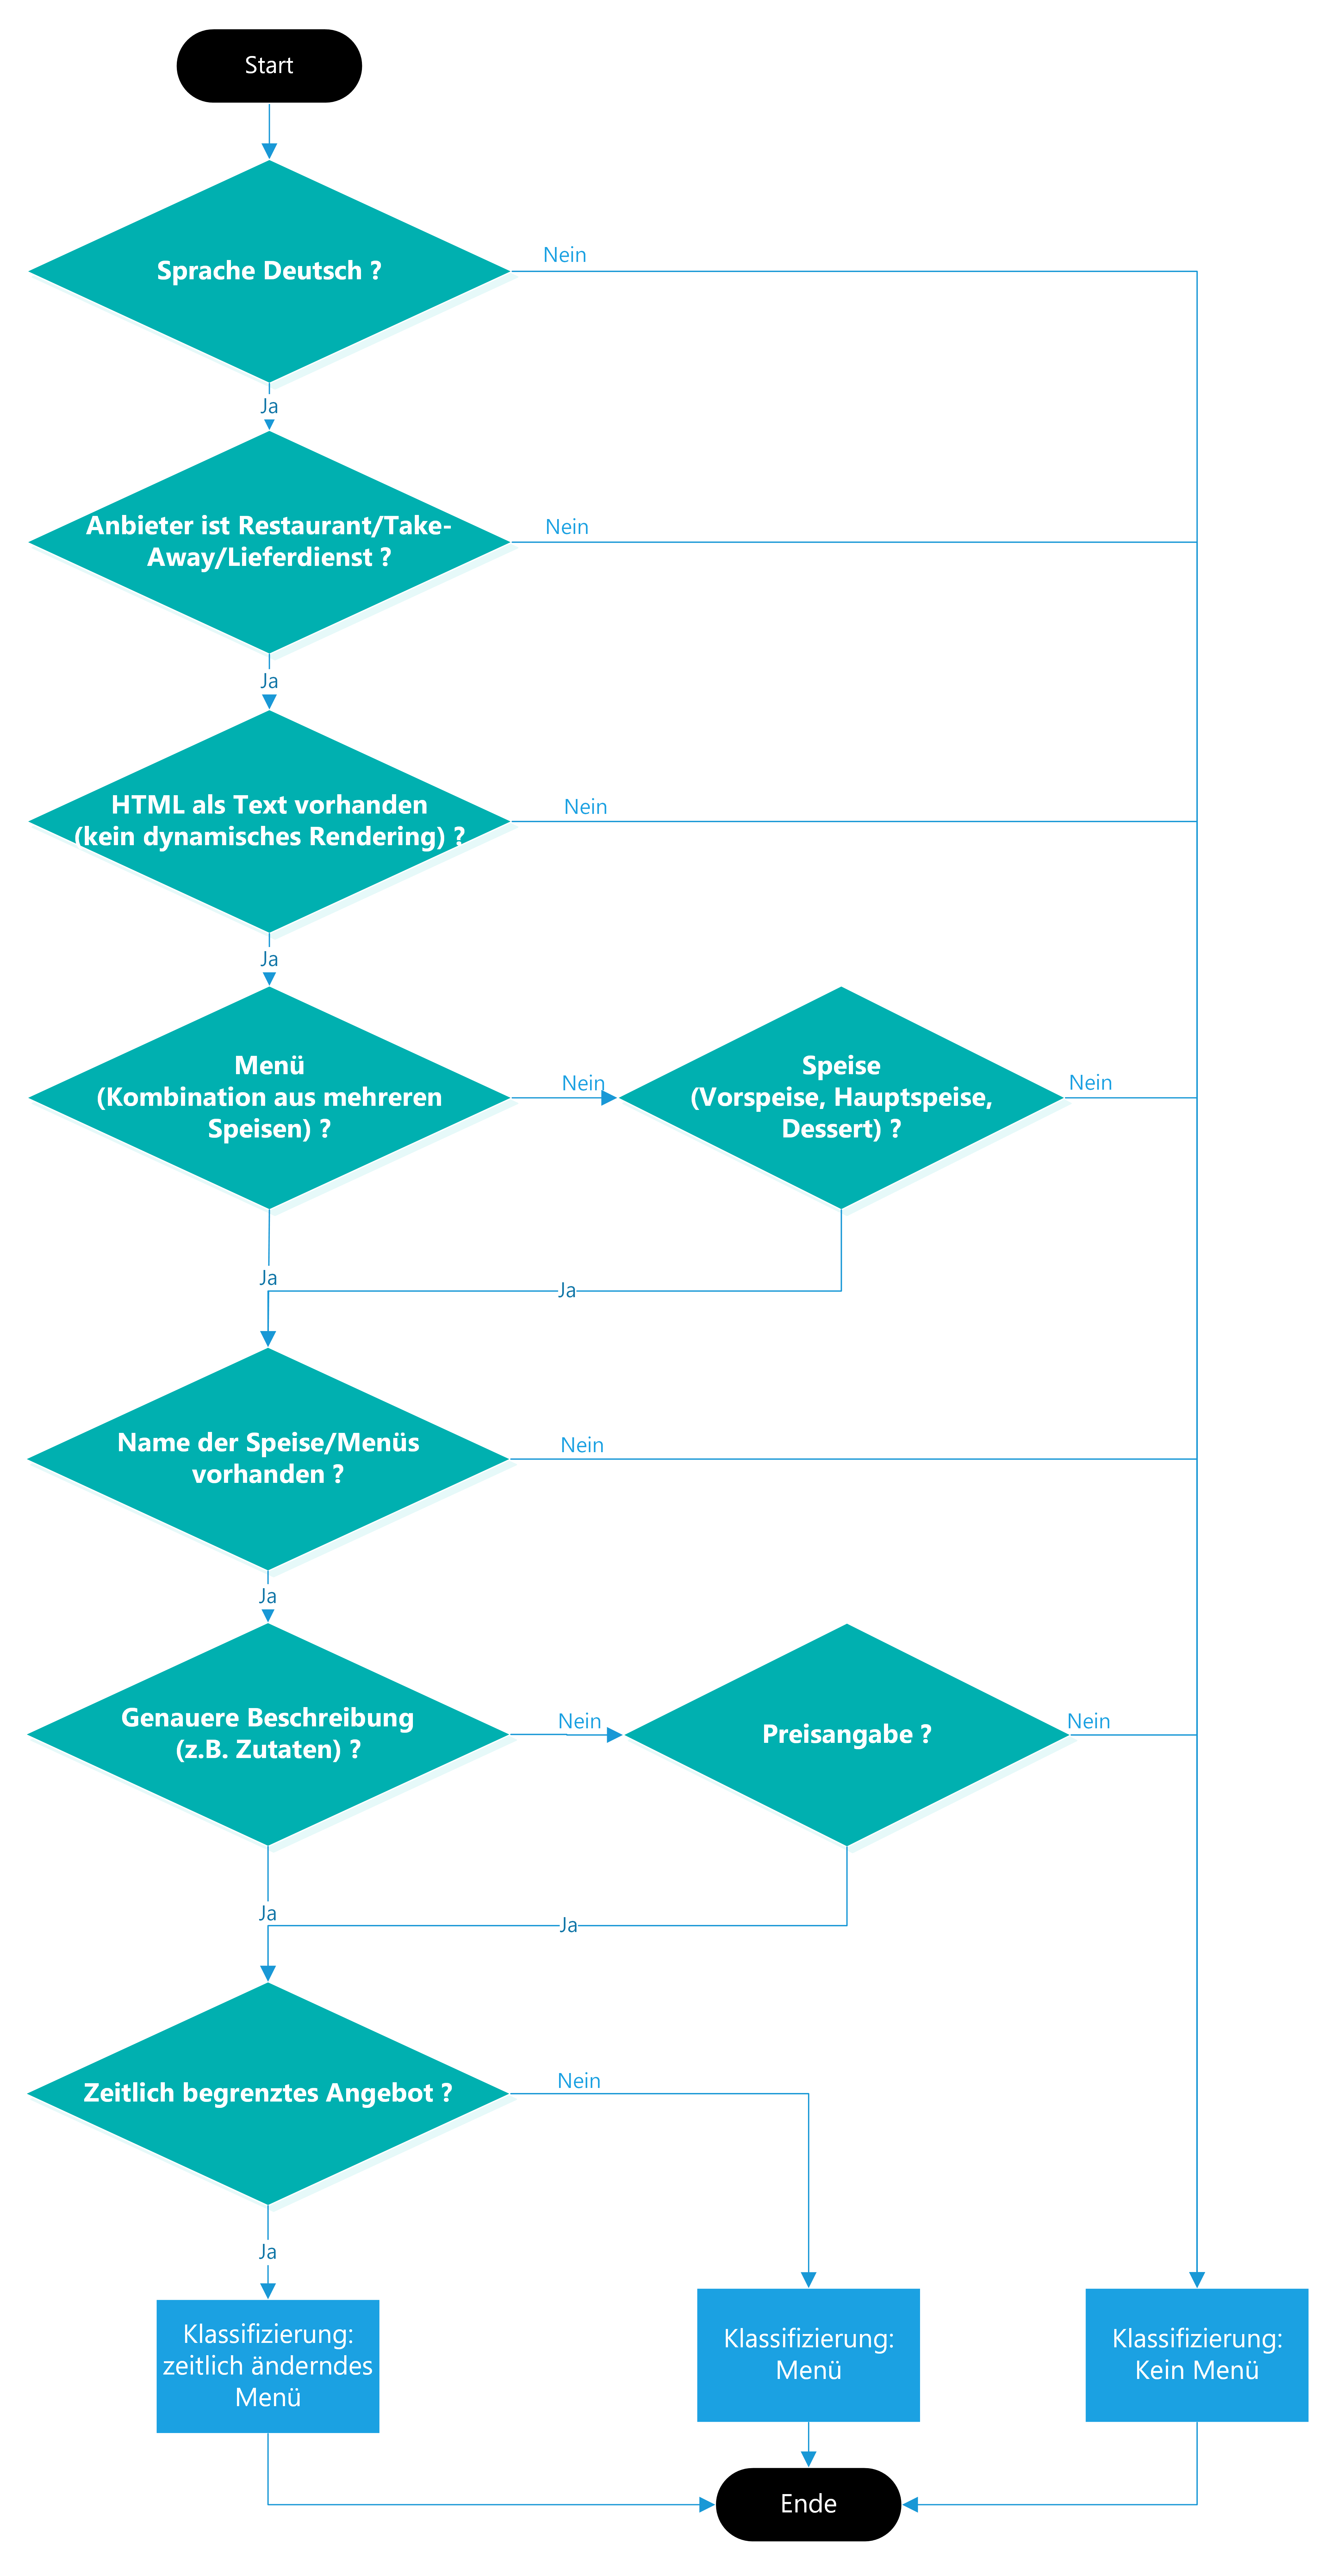
\includegraphics[width=0.65\columnwidth,keepaspectratio]{img/man-classification-tree.png}
	\caption{Entscheidungsraster}
	\label{fig:classificationtree}
\end{figure}
Obwohl bereits beim Webcrawler eine Spracherkennung eingesetzt wurde, damit nur als deutsch erkannte Webpages gespeichert werden, wurde bei der manuellen Klassifikation nochmals darauf geachtet, dass die Webpage in deutsch verfasst wurde.
Dabei ist anzumerken, dass gewisse Begriffe, vor allem für Speisebezeichnungen, auch fremdsprachig sein dürfen, da Speisebezeichnungen je nach Küche international ausgelegt sind.
Der Anbieter muss zwingend ein Restaurant, Take-Away oder Lieferdienst sein.
Der Inhalt muss statisch in der HTTP-Antwort verfügbar sein, da der Webcrawler nur diesen speichert und nicht mit dynamisch gerenderten Websites umgehen kann.
Der Name der Speise und eine genauere Beschreibung oder der Preis muss vorhanden sein.
Danach folgt die Unterscheidung zwischen zeitlich begrenzten und unbegrenzten Angeboten, welche zur Kategorisierung führt.
Getränkekarten wurden explizit negativ klassifiziert.

\section{Manuelles Labeling der Daten}
In einer ersten Durchführung des manuellen Labelings wurden ca. 1500 Dateien klassifiziert, welche das Schlüsselwort \glqq Menu\grqq{} in der URL enthalten.
Die mit dieser Heuristik gefilterten Daten entsprechen jedoch nicht einer repräsentativen Teilmenge der gesamten Rohdaten.
Darum wurde in einer zweiten Durchführung zufällig Proben aus den Rohdaten ausgewählt und manuell gelabelt.
Dadurch konnte sichergestellt werden, dass das Verhältnis von Menüseiten zu den restlichen Webpages gleich bleibt.
\subsection{Hilfsmittel: Labeling-Tool}
Um das manuelle Labeling effizienter zu gestalten, ist ein Tool\footnote{\url{https://github.com/s-santoro/testdata_tool} abgerufen am: 11.03.2019} erstellt worden, welches das Labeling vereinfacht.
Dieses Tool ruft eine Webpage der zufällig extrahierten Webpages aus den Rohdaten auf und zeigt sowohl den Text, als auch den HTML-Inhalt.
Der Anwender des Tools muss anhand dieser Informationen entscheiden, ob es sich um eine Webpage mit Menüinformationen handelt und ob diese zeitlich begrenzt sind.
Mittels Shortkeys findet die Klassifizierung statt.
Das Tool verschiebt die Datei in den entsprechenden Ordner und zeigt die Informationen der nächsten Webpage an.
\FloatBarrier
\section{Beschreibung des Gold Standards}
Der erarbeitete Gold Standard besteht insgesamt aus 6963 Dateien des Formats JSON, welche jeweils eine Webpage einer Restaurant-Website repräsentieren.
Diese Daten sind in einen Test- und einen Trainings- und Validierungsdatensatz unterteilt.
Der Gold Standard beinhaltet die folgenden drei Kategorien:
\begin{itemize}
	\item neg $\rightarrow$ Keine Menüseite
	\item pos\textunderscore daily\textunderscore menu $\rightarrow$ Zeitlich ändernde Menüseite
	\item pos\textunderscore menu $\rightarrow$ Menüseite
\end{itemize}
Die Datenstruktur des Gold Standards sieht wie folgt aus:\\

\begin{forest}
	for tree={
		font=\ttfamily,
		grow'=0,
		child anchor=west,
		parent anchor=south,
		anchor=west,
		calign=first,
		edge path={
			\noexpand\path [draw, \forestoption{edge}]
			(!u.south west) +(7.5pt,0) |- node[fill,inner sep=1.25pt] {} (.child anchor)\forestoption{edge label};
		},
		before typesetting nodes={
			if n=1
			{insert before={[,phantom]}}
			{}
		},
		fit=band,
		before computing xy={l=15pt},
	}
	[Gold Standard (6963 Dateien)
	[test (100 Dateien)
	[neg (50 Dateien)]
	[pos\textunderscore daily\textunderscore menu (10 Dateien)]
	[pos\textunderscore menu (40 Dateien)]
	]
	[train-validation (6863 Dateien)
	[neg (6257 Dateien)]
	[pos\textunderscore daily\textunderscore menu (87 Dateien)]
	[pos\textunderscore menu (519 Dateien)]
	]
	]
\end{forest}\\


Jeder Eintrag dieses Gold Standards beinhaltet die folgenden Informationen:
\begin{itemize}
	\item \glqq date\grqq{} - Zeitpunkt, zu welchem die Webpage aufgerufen wurde
	\item \glqq text\grqq{} - Vom Webcrawler extrahierter Text, welcher die Webpage beinhaltet
	\item \glqq encoding\grqq{} - Das von der Webpage verwendete Encoding
	\item \glqq title\grqq{} - Inhalt des gleichnamigen HTML-Metatags
	\item \glqq url\grqq{} - URL der Webpage
	\item \glqq content\grqq{} - Der statische HTML-Inhalt der Webpage	
\end{itemize}



\newpage

\chapter{Experiment und Klassifizierung}
\label{cap:exp_class}
Sämtliche Klassifikation findet anhand der Informationen der Attribute \glqq text \grqq und \glqq title \grqq des Gold Standards statt.
Zudem werden alle Webpages der Kategorie \glqq Tagesmenü \grqq der Kategorie \glqq Menü \grqq hinzugefügt, da bei dieser Klassifikation nur zwischen \glqq Menü \grqq oder \glqq Kein Menü \grqq unterschieden wird.
\section{Regelbasiertes Klassifizieren}
Jedes Regelset wurde anhand des Goldstandards getestet und evaluiert.
Verschiedene Parameterwerte und Kombinationen wurden getestet, um möglichst hohe Werte der gemessenen Metriken zu erreichen.
Bei allen Regelsets sind alle Methoden des Preprocessings aktiv gewesen. 
\subsection{Regelset: Menü im Titel}
Für dieses Regelset sind keine Parameter verfügbar, daher ist nur eine Konfiguration durchgeführt worden.
Diese hat folgende Metriken ergeben:\\
\begin{table}[H]
\caption{Score des Regelsets: Menü im Titel}
\centering
\begin{tabular}{|l|l|l|}
	\hline
	F1-Score & Precision & Recall\\
	\hline
	0.17 & 0.43 & 0.11  \\
	\hline
\end{tabular}
\end{table}
\subsection{Regelset: Preisdetektor}
Durch die Konfiguration kann ein Schwellwert für die Anzahl erkannter Preise angegeben werden, die vorhanden sein müssen, um eine Webpage als positiv zu klassifizieren.\\
\begin{table}[H]
\caption{Scores des Regelsets: Preisdetektor}
\centering
\begin{tabular}{|l|l|l|l|}
	\hline
	Schwellwert & F1-Score & Precision & Recall\\
	\hline
	1 & 0.45 & 0.36 & 0.60  \\
	2 & 0.46 & 0.45 & 0.47 \\
	3 & 0.41 & 0.49 & 0.36 \\
	\hline
\end{tabular}
\end{table}
Das beste Ergebnis hat ein Schwellwert von zwei erzielt, danach ist der F1-Score wieder schlechter geworden.
Daraus wurde geschlussfolgert, dass für dieses Regelset das Maximum bereits erreicht wurde.
\subsection{Regelset: Kombination aus Menü im Titel und Preisdetektor}
Bei dieser Konfiguration kann der Schwellwert ebenfalls für die Anzahl erkannter Preise angegeben werden.\\
\begin{table}[H]
	\caption{Scores des Regelsets: Kombination aus Menü im Titel und Preisdetektor}
	\centering
\begin{tabular}{|l|l|l|l|}
	\hline
	Schwellwert & F1-Score & Precision & Recall\\
	\hline
	1 & 0.45 & 0.35 & 0.65 \\
	2 & 0.47 & 0.43 & 0.52 \\
	3 & 0.43 & 0.45 & 0.41 \\
	\hline
\end{tabular}
\end{table}
Auch bei diesem Regelset hat die Konfiguration mit einem Schwellwert von zwei das beste Ergebnis erzielt.
\subsection{Regelset: Listing}
Beim Listing können zwei Schwellwerte angeben werden, einen für die Anzahl übereinstimmender Wörter aus der Whitelist und einen für die Blacklist.
In einem ersten Versuch wurden identische Schwellwerte gewählt und jeweils erhöht:\\
\begin{table}[H]
	\caption{Scores der ersten Iteration des Regelsets: Listing}
	\centering
\begin{tabular}{|l|l|l|l|l|}
	\hline
	Schwellwert Whitelist & Schwellwert Blacklist & F1-Score & Precision & Recall\\
	\hline
	1 & 1 & 0.17 & 0.32 & 0.11 \\
	5 & 5 & 0.39 & 0.62 & 0.29 \\
	10 & 10 & 0.42 & 0.77 & 0.29 \\
	20 & 20 & 0.33 & 0.85 & 0.21 \\
	30 & 30 & 0.27 & 0.91 & 0.16 \\
	\hline
\end{tabular}
\end{table}
Dieser Versuch hat gezeigt, dass ein maximaler F1-Score bei gleichen Werten zwischen 5 und 20 zu erreichen ist.\\
Da gleich gewählte Werte keine zufriedenstellende Ergebnisse erzielten, wurden im zweiten Versuch unterschiedliche Verhältnisse getestet:\\
\begin{table}[H]
	\caption{Scores der zweiten Iteration des Regelsets: Listing}
	\centering
\begin{tabular}{|l|l|l|l|l|}
	\hline
	Schwellwert Whitelist & Schwellwert Blacklist & F1-Score & Precision & Recall\\
	\hline
	5 & 1 & 0.12 & 0.82 & 0.07 \\
	1 & 5 & 0.31 & 0.24 & 0.45 \\
	\hline
\end{tabular}
\end{table}
Aus diesem Versuch entstand die Schlussfolgerung, dass ein höherer Schwellwert der Blacklist als der Whitelist erforderlich ist, um einen möglichst hohen Score zu erreichen.
Diese Erkenntnis wurde in einem weiteren Versuch in mehreren Iterationen getestet:\\
\begin{table}[H]
	\caption{Scores der dritten Iteration des Regelsets: Listing}
	\centering
\begin{tabular}{|l|l|l|l|l|}
	\hline
	Schwellwert Whitelist & Schwellwert Blacklist & F1-Score & Precision & Recall\\
	\hline
	2 & 10 & 0.42 & 0.33 & 0.61 \\
	3 & 15 & 0.52 & 0.42 & 0.70 \\
	3 & 20 & 0.51 & 0.39 & 0.75 \\
	4 & 15 & 0.53 & 0.47 & 0.61 \\
	5 & 15 & 0.55 & 0.54 & 0.56 \\
	5 & 20 & 0.54 & 0.50 & 0.60 \\
	5 & 21 & 0.54 & 0.49 & 0.60 \\
	6 & 20 & 0.55 & 0.56 & 0.55 \\
	7 & 20 & 0.55 & 0.60 & 0.50 \\
	8 & 20 & 0.53 & 0.64 & 0.46 \\
	\hline
\end{tabular}
\end{table}
Die Schwellwerte wurden stetig erhöht.
Verschiedene Schwellwerte in unterschiedlichen Verhältnissen wurden dabei getestet.
Sobald einer dieser Schwellwerte zu einem schlechteren Ergebnis geführt hat, wurde er wieder reduziert oder ein neues Verhältnis wurde getestet.
Beim Verhältnis 6/20 bzw. 7/20 wurde das Maximum des F1-Scores erreicht.
Da diese Werte nicht im Bereich einer brauchbaren Klassifikation sind, wurde auf das Ermitteln aller möglichen Kombinationen verzichtet.
\subsection{Regelset: Bag of Words}
Bei diesem Regelset kann die Grösse der Black- und Whitelist (Features), das Verhältnis zwischen Test- und Trainingsdaten (Split) sowie ein Schwellwert angegeben werden.
Für das Verhältnis zwischen Test- und Trainingsdaten wurden die Werte 0.3, 0.5 und 0.7 getestet.
In einer ersten Iteration wurde die Anzahl von 200 Features und ein Split von 0.3 verwendet, um herauszufinden, ob ein positiver oder negativer Schwellwert bessere Werte erzielt.\\
\begin{table}[H]
	\caption{Scores der ersten Iteration des Regelsets: Bag of Words}
	\centering
\begin{tabular}{|l|l|l|l|}
	\hline
	Schwellwert & F1-Score & Precision & Recall\\
	\hline
	0 & 0.64 & 0.58 & 0.71 \\
	2 & 0.51 & 0.38 & 0.75 \\
	-2 & 0.68 & 0.74 & 0.63 \\
	\hline
\end{tabular}
\end{table}
Dabei wurde erkannt, dass sich ein negativer Schwellwert positiv auf den F1-Score auswirkt.\\
In der zweiten Iteration wurde der Schwellwert weiter verkleinert.\\
\begin{table}[H]
	\caption{Scores der zweiten Iteration des Regelsets: Bag of Words}
	\centering
\begin{tabular}{|l|l|l|l|}
	\hline
	Schwellwert & F1-Score & Precision & Recall\\
	\hline
	-3 & 0.66 & 0.80 & 0.57 \\
	-4 & 0.66 & 0.86 & 0.54 \\
	-5 & 0.66 & 0.89 & 0.52 \\
	\hline
\end{tabular}
\end{table}\
Da diese Werte sich fast nicht unterscheiden, wurden alle weiterverwendet, um einen maximalen Score zu evaluieren.
In einer dritten, ausführlicheren Iteration sind die Anzahl Features von 200 bis 400 sowie die drei oben genannten Verhältnisse zusammen mit den vier Schwellwerten getestet worden. Die folgende Tabelle zeigt diese Tests, sortiert nach bestem F1-Score:\\
\begin{table}[H]
	\caption{Scores der dritten Iteration des Regelsets: Bag of Words}
	\centering
\begin{tabular}{ | l | l | l | l | l | l | }
	\hline
	Split & Features & Limit & F1 & Pre & Rec \\ \hline
	0.3 & 400 & -3 & 0.72 & 0.74 & 0.7 \\ 
	0.3 & 400 & -4 & 0.72 & 0.79 & 0.66 \\
	0.3 & 400 & -5 & 0.72 & 0.81 & 0.64 \\
	0.7 & 400 & -3 & 0.72 & 0.75 & 0.69 \\
	0.7 & 400 & -4 & 0.72 & 0.79 & 0.66 \\
	0.5 & 300 & -3 & 0.71 & 0.79 & 0.65 \\
	0.5 & 400 & -3 & 0.70 & 0.74 & 0.67 \\
	0.5 & 400 & -4 & 0.70 & 0.79 & 0.63 \\ 
	0.7 & 400 & -2 & 0.70 & 0.70 & 0.70 \\ 
	0.7 & 300 & -3 & 0.70 & 0.74 & 0.67 \\
	0.7 & 300 & -4 & 0.70 & 0.80 & 0.63 \\
	0.7 & 300 & -5 & 0.70 & 0.84 & 0.60 \\
	0.7 & 400 & -5 & 0.70 & 0.82 & 0.62 \\ 
	0.3 & 400 & -2 & 0.69 & 0.66 & 0.73 \\ 
	0.5 & 400 & -2 & 0.69 & 0.69 & 0.69 \\ 
	0.5 & 400 & -5 & 0.69 & 0.82 & 0.60 \\ 
	0.7 & 200 & -3 & 0.69 & 0.76 & 0.63 \\ 
	0.7 & 200 & -4 & 0.69 & 0.81 & 0.60 \\ 
	0.3 & 300 & -2 & 0.68 & 0.73 & 0.64 \\ 
	0.3 & 300 & -3 & 0.68 & 0.78 & 0.60 \\ 
	0.3 & 200 & -2 & 0.68 & 0.74 & 0.63 \\ 
	0.5 & 200 & -3 & 0.68 & 0.77 & 0.60 \\ 
	0.5 & 300 & -4 & 0.68 & 0.81 & 0.59 \\ 
	0.7 & 300 & -2 & 0.68 & 0.69 & 0.68 \\ 
	0.5 & 200 & -2 & 0.67 & 0.71 & 0.64 \\ 
	0.3 & 300 & -4 & 0.66 & 0.82 & 0.56 \\ 
	0.3 & 200 & -3 & 0.66 & 0.80 & 0.57 \\
	0.3 & 200 & -4 & 0.66 & 0.86 & 0.54 \\
	0.3 & 200 & -5 & 0.66 & 0.89 & 0.52 \\ 
	0.5 & 200 & -4 & 0.66 & 0.81 & 0.56 \\
	0.5 & 300 & -5 & 0.66 & 0.83 & 0.55 \\ 
	0.7 & 200 & -2 & 0.66 & 0.66 & 0.66 \\ 
	0.7 & 200 & -5 & 0.66 & 0.85 & 0.55 \\ 
	0.3 & 300 & -5 & 0.65 & 0.85 & 0.52 \\ 
	0.5 & 200 & -5 & 0.65 & 0.87 & 0.52 \\
	0.5 & 300 & -2 & 0.46 & 0.62 & 0.36 \\ \hline
\end{tabular}
\end{table}
Daraus lässt sich schliessen, dass eine hohe Anzahl Features zu einem besseren Ergebnis führt.
Das Verhältnis zwischen Test- und Trainingsdaten ist nicht so relevant, da sowohl das Verhältnis 0.3 als auch 0.7 zu hohen Scores führt.
Der Schwellwert ist im Bereich -2 bis -5 ebenfalls nicht aussagekräftig, da auch dieser bei den besten Scores vertreten ist.
Es muss zudem berücksichtigt werden, dass der Split zufällig gewählt wird und keine Kreuzvalidierung stattfindet, dadurch können diese Ergebnisse variieren.
\section{Auswirkungen des Preprocessings}
\subsection{Regelbasiertes Klassifizieren}
Bei den Methoden des regelbasierten Klassifizierens trägt das Preprocessing einen erheblichen Teil zum Erfolg bei.
Die Methode \glqq Menü im Titel\grqq{} profitiert davon, dass Umlaute mit den entsprechenden Selbstlauten ersetzt werden.
Der Preisdetektor funktioniert ohne den gleichnamigen Preprocessingschritt gar nicht, da nach dem Ersatzwort gesucht wird.
Beide Punkte gelten auch für die Kombination dieser Methoden.\\
Das Listing profitiert von mehreren Preprocessingschritten.
Das Ersetzen der Grossbuchstaben durch Kleinbuchstaben, der Preis- und Getränkedetektor sowie die Stammformreduktion führen dazu, dass im Text vorkommende Worte den Worten der jeweiligen Listen besser zugeordnet werden können.
Die Methode \glqq Bag of Words\grqq{} profitiert davon ebenfalls, da das Prinzip dasselbe ist.\\
Es können keine genauen Zahlen angegeben werden, welche Scores diese Methoden ohne Preprocessingschritte erreichen würden, da diese Schritte zwingend benötigt werden, um den Text in eine klassifizierbare Form zu bringen.
\subsection{Klassifizieren mittels Machine-Learning}
\subsubsection{Einfache Preprocessingschritte}
Das Anwenden von einfachen Preprocessingschritten hat bei allen drei Feature-Extraction Methoden Verbesserungen bewirkt.\\
Lediglich bei der TF-IDF Methode verschlechterten sich gewisse Algorithmen mit dem einfachen Preprocessing.
Die Verbesserungen beim TF-IDF sind jedoch markanter als die Verschlechterungen.\\
Das einfache Preprocessing hatte auf alle drei Varianten positive Einwirkungen und wird somit auch bei allen dreien weiter verwendet.
\begin{figure}[H]	
	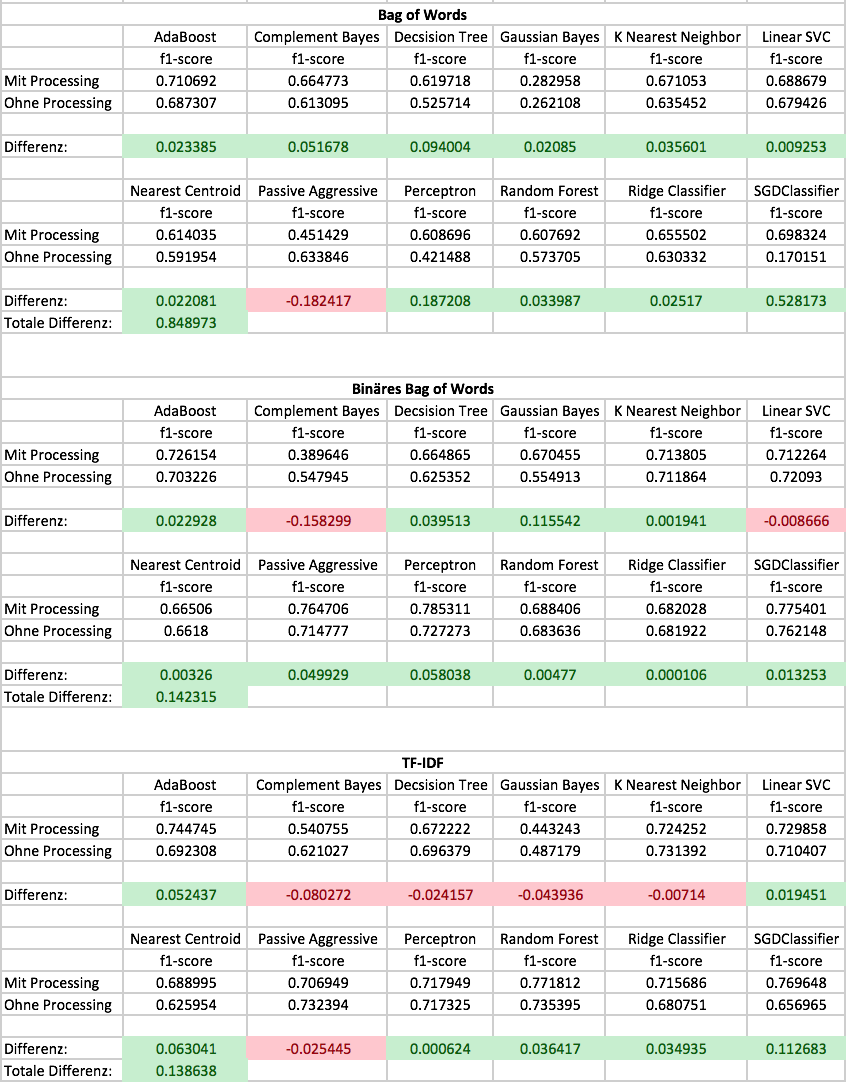
\includegraphics[width=1\columnwidth,keepaspectratio]{img/easypre.png}
	\caption{Grafik der Auswertung für einfaches Preprocessing}
\end{figure}
\subsubsection{Fortschrittliche Preprocessingschritte}
Das fortschrittliche Preprocessing erzielt bei allen drei Feature-Extraction Methoden keine eindeutigen Resultate.\\
Bei der \glqq Bag of Words\grqq{} Methode erreicht die Konfiguration \glqq config8\grqq{} mit dem Preisdetektor, der Stoppwörterentfernung und der Stammformreduktion die grössten positiven Einwirkungen.
Sieben Algorithmen können mit dieser Konfiguration ihre F1-Scores verbessern.
Somit wird für \glqq Bag of Words\grqq{} die Konfiguration \glqq config8\grqq{} weiter benutzt.\\
Bei der binären \glqq Bag of Words\grqq{} Methode gibt es bei keiner Konfiguration irgendwelche flächendeckenden Verbesserungen.
Es gibt jeweils nur vereinzelte Algorithmen, welche ihre Scores verbessern können.
Da keine Konfiguration eindeutig als Verbesserung angesehen werden kann, wird bei dieser Variante keine fortschrittlichen Preprocessingschritte angewendet.\\
Bei der TF-IDF-Methode gibt es ebenfalls keine eindeutigen Verbesserungen bei irgendeiner Konfiguration.
Es können vereinzelte Algorithmen ihre Scores verbessern, aber es findet nie flächendeckend eine Verbesserung statt.
Bei der Konfiguration \glqq config5\grqq{} erzielt AdaBoost den höchsten Wert über alle Konfigurationen gesehen, aber die anderen Algorithmen werden nur leicht beeinflusst.
Um bei der weiteren Ermittlung von Optimierungen nicht nur auf ein Algorithmus zu setzen, wird bei TF-IDF kein fortschrittliches Preprocessing angewendet.
\\\\
Die Auswertung für das fortschrittliche Preprocessing kann im Anhang gefunden werden.
\section{Klassifizieren mittels Machine-Learning}
\subsection{Dimensionsreduktion der Features}
Die Verwendung der Dimensionsreduktion mittels LSA erzielt bei allen drei Feature-Extraction Methoden deutliche Verbesserungen.
Der Grossteil der Algorithmen kann mit Hilfe von LSA den F1-Score verbessern.
Lediglich bei der \glqq Bag of Words\grqq{} Methode ist die Summe über alle Score-Verbesserungen negativ, dies jedoch nur, weil der Multinomial-Bayes Klassifizierer mit LSA einen stetigen F1-Score von null hat.\\
Die Dimensionsreduktion wird für alle drei Varianten weiter verwendet, da die positiven Auswirkungen sich deutlich in den F1-Scores widerspiegelt.
Einziger Wehrmutstropfen der Dimensionsreduktion ist, dass der Multinomial-Bayes Klassifizierer keine wirkliche Klassifizierung mehr durchführen kann.
Somit ist dieser Klassifizierer für den weiteren Verlauf nicht mehr verwendbar.
\begin{figure}[H]	
	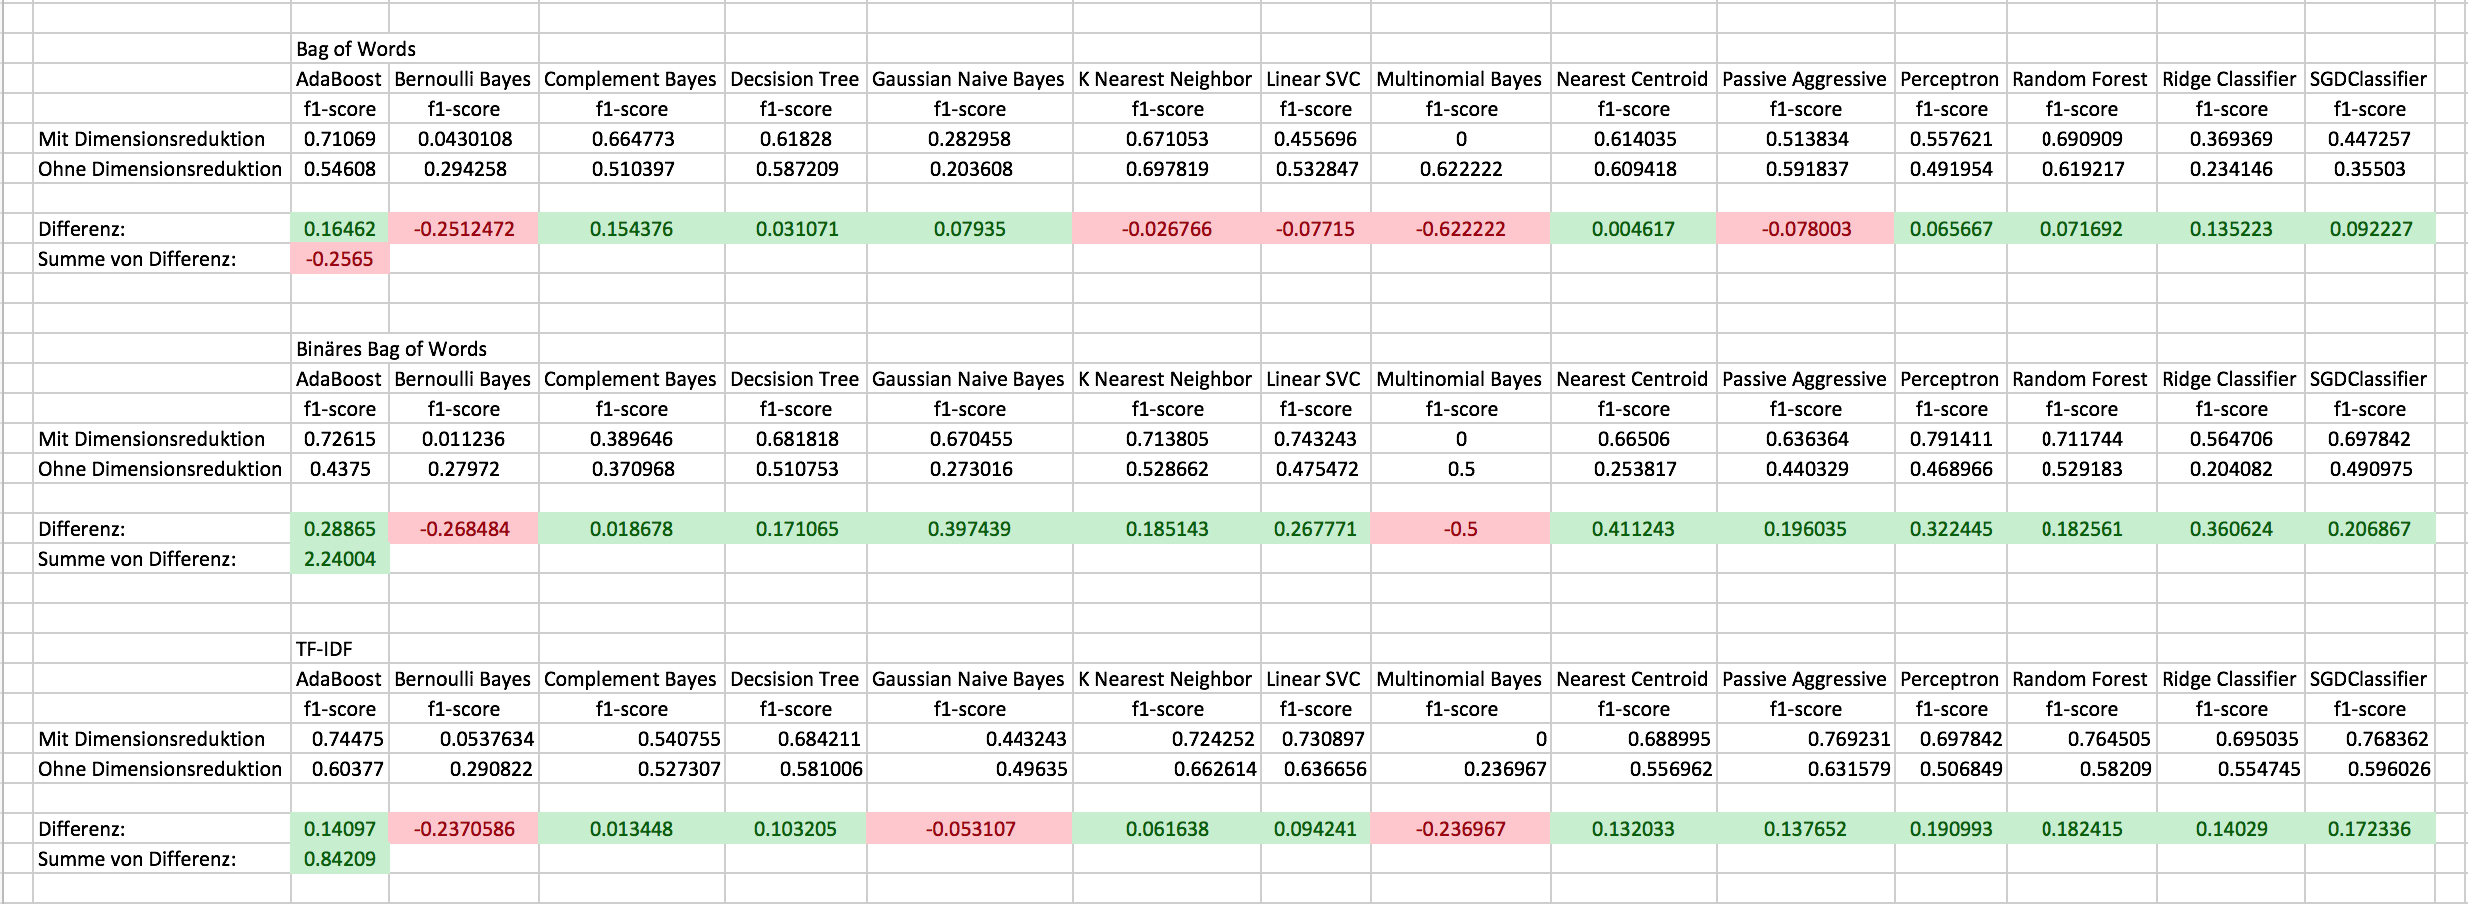
\includegraphics[width=1\columnwidth,keepaspectratio]{img/dimred.png}
	\caption{Grafik der Auswertung für die Dimensionsreduktion mittels LSA}
\end{figure}
\subsection{Klassenverteilung}
Die Angabe der Klassenverteilung konnte nicht bei allen Algorithmen als Parameter angegeben werden.
Somit werden alle Bayes-Algorithmen, KNearestNeighbor und Nearest-Centroid in dieser Auswertung nicht beachtet.\\
Bei beiden \glqq Bag of Words\grqq{} Methoden erzielt die Angabe der Klassenverteilung eine durchschnittliche Verbesserung der F1-Scores.
Einzelne Algorithmen reagieren negativ auf die Angabe, aber die positiven Auswirkungen übertreffen die negativen Auswirkungen.
Somit wird bei beiden \glqq Bag of Words\grqq{} Methoden die Angabe der Klassenverteilung miteinbezogen.\\
Bei der TF-IDF-Methode werden drei Algorithmen negativ und vier Algorithmen positiv beeinflusst.
Lediglich beim PassiveAgressiveClassifier gibt es eine markante Verschlechterung des F1-Scores.
Bei den anderen Algorithmen halten sich die negativen Auswirkungen im Rahmen.
Den F1-Score des PassiveAgressiveClassifier ausgenommen, sind die positiven Auswirkungen grösser als die negativen Auswirkungen.
Somit wird für TF-IDF ebenfalls die Angabe der Klassenverteilung für die nächsten Schritte beibehalten.
\begin{figure}[H]	
	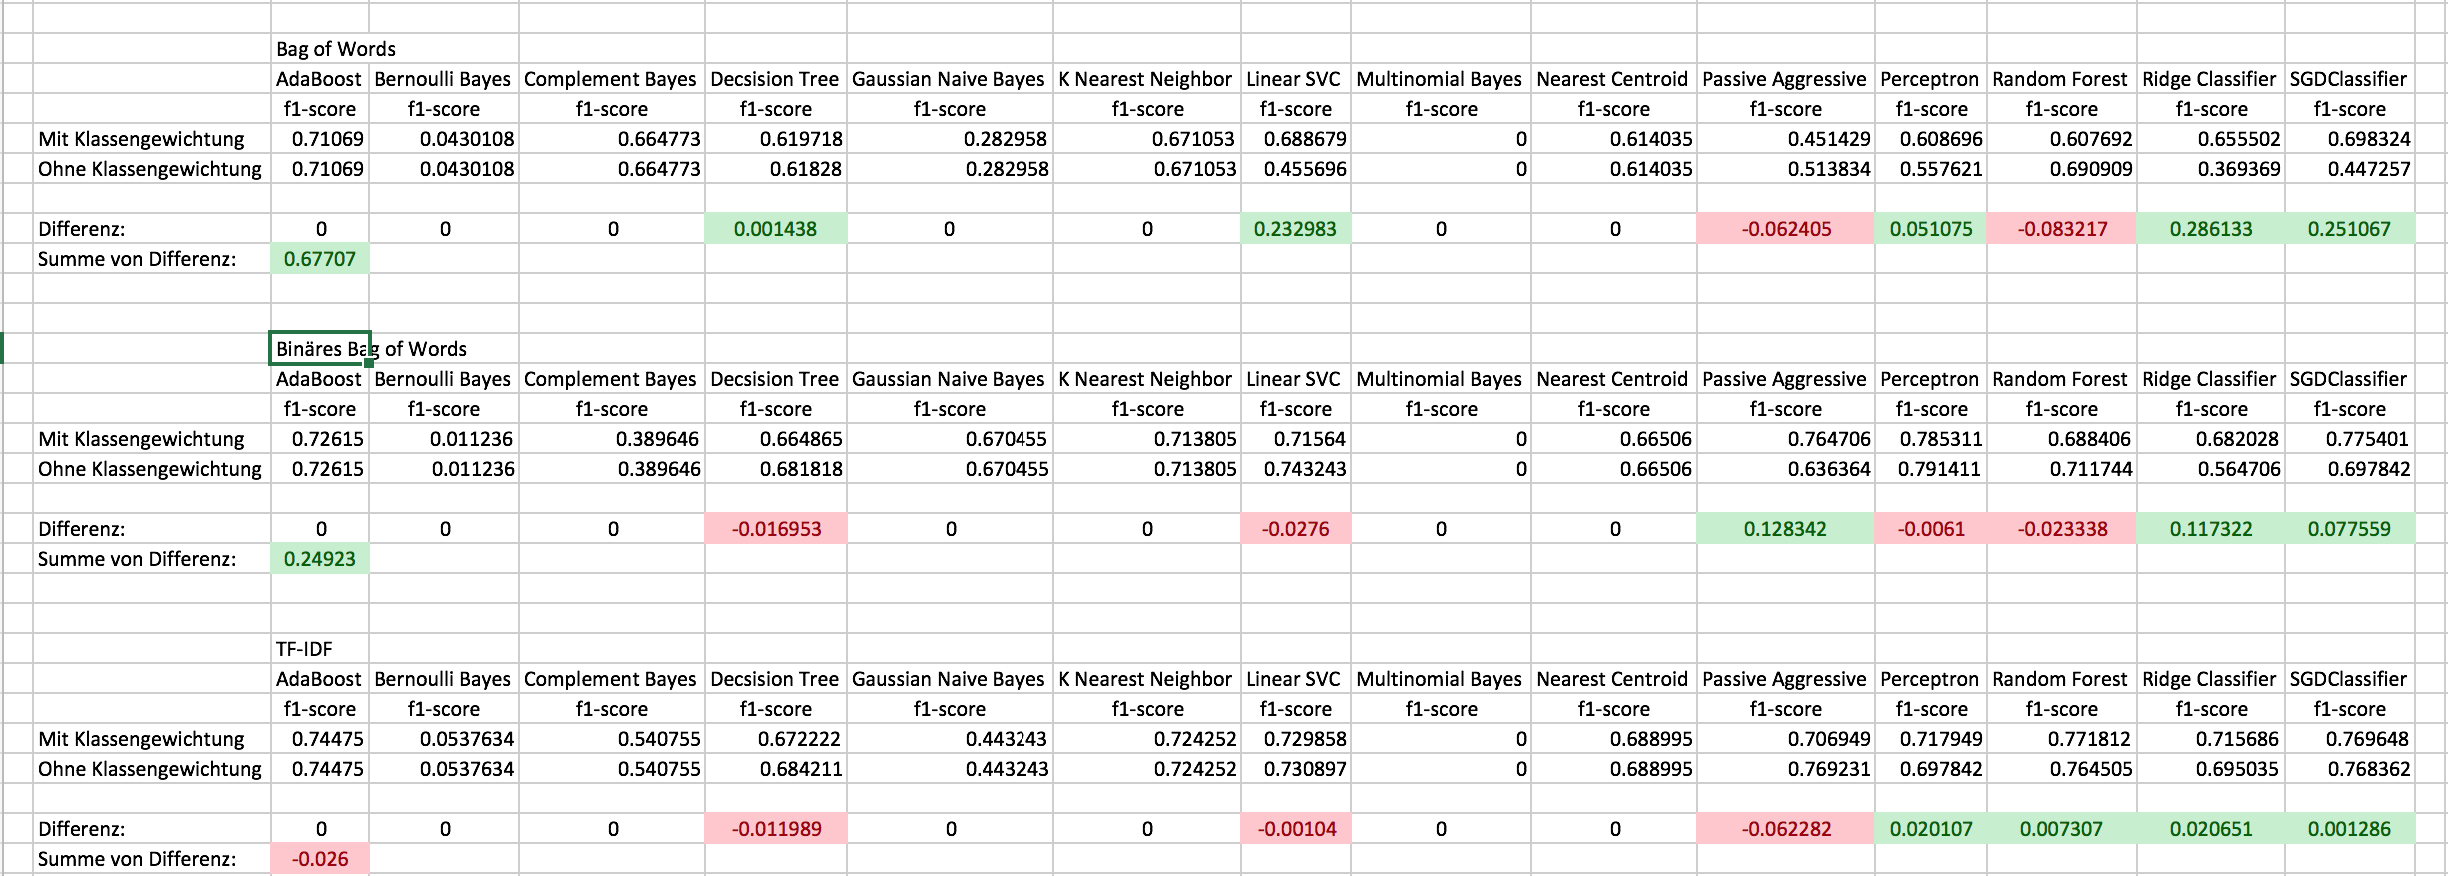
\includegraphics[width=1\columnwidth,keepaspectratio]{img/classweight.png}
	\caption{Grafik der Auswertung für die Klassenverteilung}
\end{figure}
\subsection{N-Gramme}
Sowohl \glqq Bag of Words\grqq{} als auch TF-IDF bieten in ihrer Scikit-Learn Implementierung die Möglichkeit N-Gramme zu verwenden.
Für dieses Experiment wurden Unigramme, Bigramme und Trigramme ausgetestet.\\
Bei beiden \glqq Bag of Words\grqq{} Methoden erzielt die Verwendung von Unigrammen die besten Ergebnisse.
Bi- und Trigramme können bei einzelnen Algorithmen ebenfalls eine Verbesserunge verzeichnen, aber im Vergleich zu Unigrammen fallen diese flächendeckend kleiner aus.
Somit werden bei beiden \glqq Bag of Words\grqq{} Varianten nur Unigramme verwendet.
Ebenfalls benötigt die Extrahierung der Features bei Bi- und Trigrammen circa doppelt so lange, was eine enorme Performanceeinbusse ist.\\
Bei der TF-IDF-Methode erzielen Bi- und Trigramme die exakt gleichen Werte.
Uni- und Bigramme erzielen im Durchschnitt ungefähr den gleichen Wert.
Bei der Verwendung von Unigrammen erzielt der Algorithmus Bernoulli-Bayes einen F1-Score von null.
Um nicht einen weiteren Algorithmus für die weiteren Schritte zu verlieren, wird deshalb die Verwendung von Bigrammen bei der TF-IDF-Methode verwendet.
\begin{figure}[H]	
	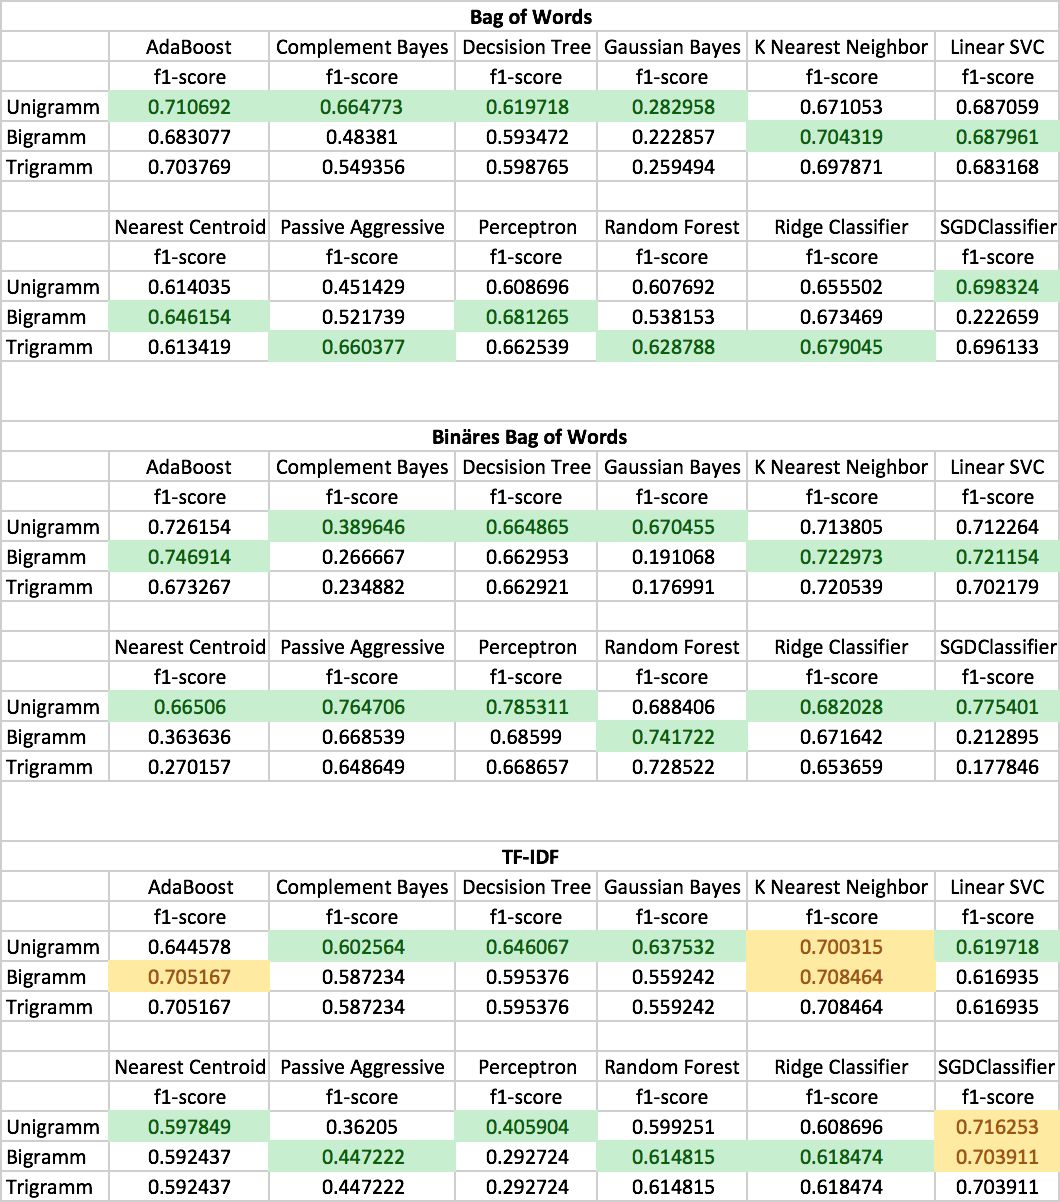
\includegraphics[width=1\columnwidth,keepaspectratio]{img/ngram.png}
	\caption{Grafik der N-Gramme Auswertung}
\end{figure}
\subsection{Anzahl extrahierter Features}
Für alle drei Feature-Extraction Methoden wurde ein Liniendiagramm für F1-Score, Precision und Recall erstellt.
Aus diesen Grafiken kann entnommen werden, bei welcher Feature-Anzahl welcher Algorithmus den besten Score erzielt.
Für die weitere Auswertung sind die Grafiken für F1-Score und Precision massgebend und werden weiter analysiert.
\subsubsection{Bag of Words}
Bei \glqq Bag of Words\grqq{} erzielt der Algorithmus AdaBoost bei 100 Features mit Abstand den besten F1-Score und erreicht fast die 0.8 Marke.
Ebenfalls kann der LinearSVC Algorithmus einen guten F1-Score erzielen und teilt sich mit AdaBoost die besten Werte.
Ersichtlich ist ebenfalls, dass die meisten Algorithmen sich zwischen 0.6 und 0.7 bewegen und das vereinzelte Klassifizierer mit ihren Werten auf und ab springen.\\
\begin{figure}[H]	
	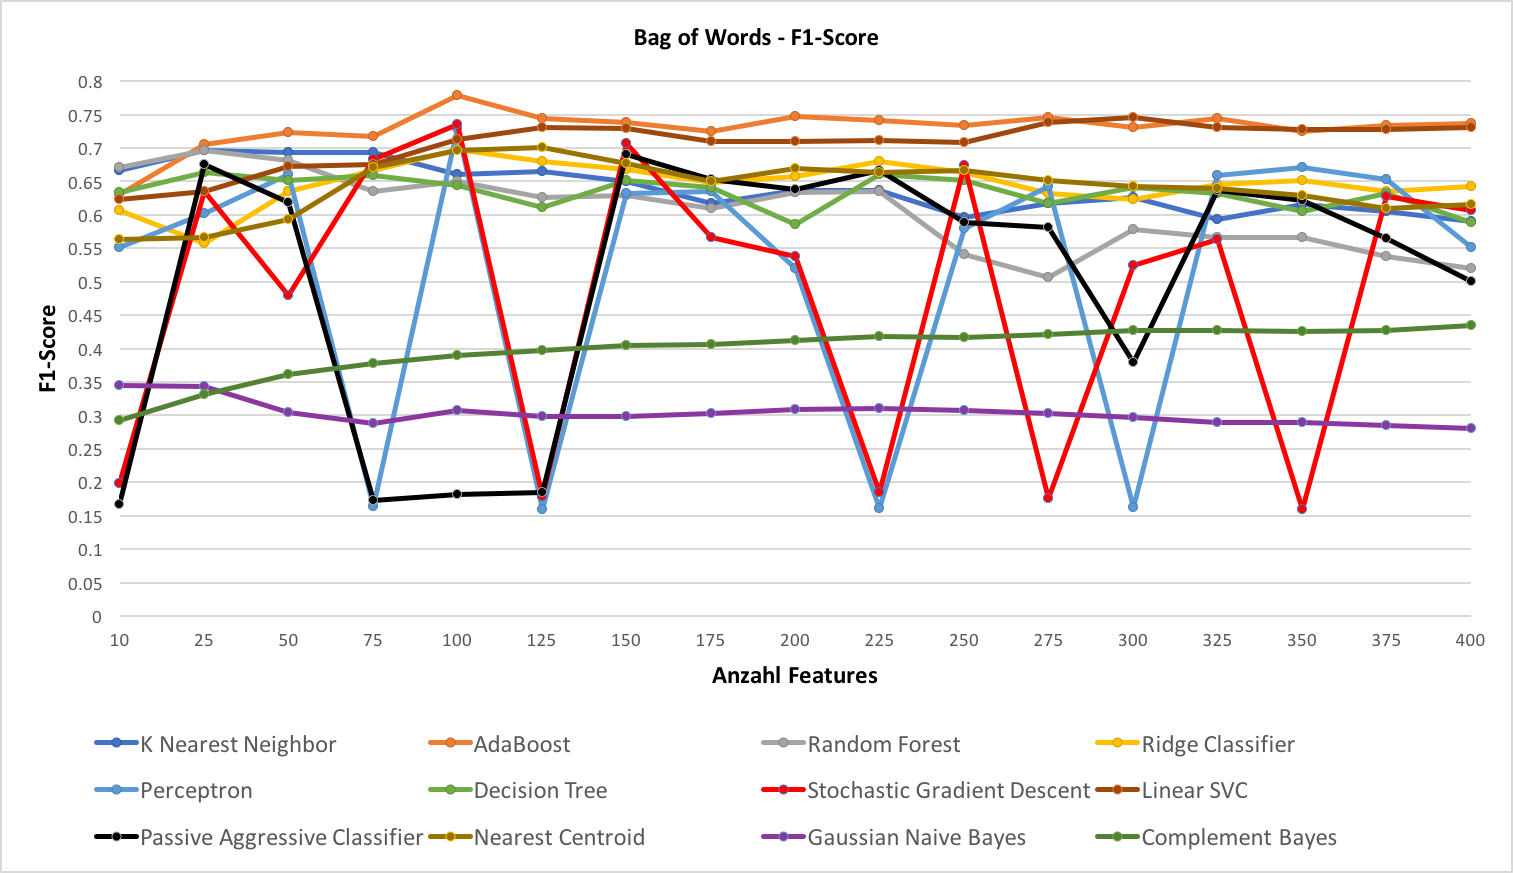
\includegraphics[width=0.8\columnwidth,keepaspectratio]{img/bow-f1.png}
	\caption{Grafik des F1-Score-Verlaufs bei Bag of Words}
\end{figure}
Bei der Precision ist der RandomForest Algorithmus der mit Abstand beste Klassifizierer.
Vereinzelt erreicht RandomForest eine Precision von 1.0 und ist stetig über 0.8.\\
Der Bernoulli-Bayes Algorithmus erreicht kurzzeitig ebenfalls eine Precision von eins, jedoch ist sein F1-Score jeweils unter 0.1.
Deswegen wir Bernoulli-Bayes nicht als ernsthafte Wahl angesehen und nicht beachtet.
\begin{figure}[H]	
	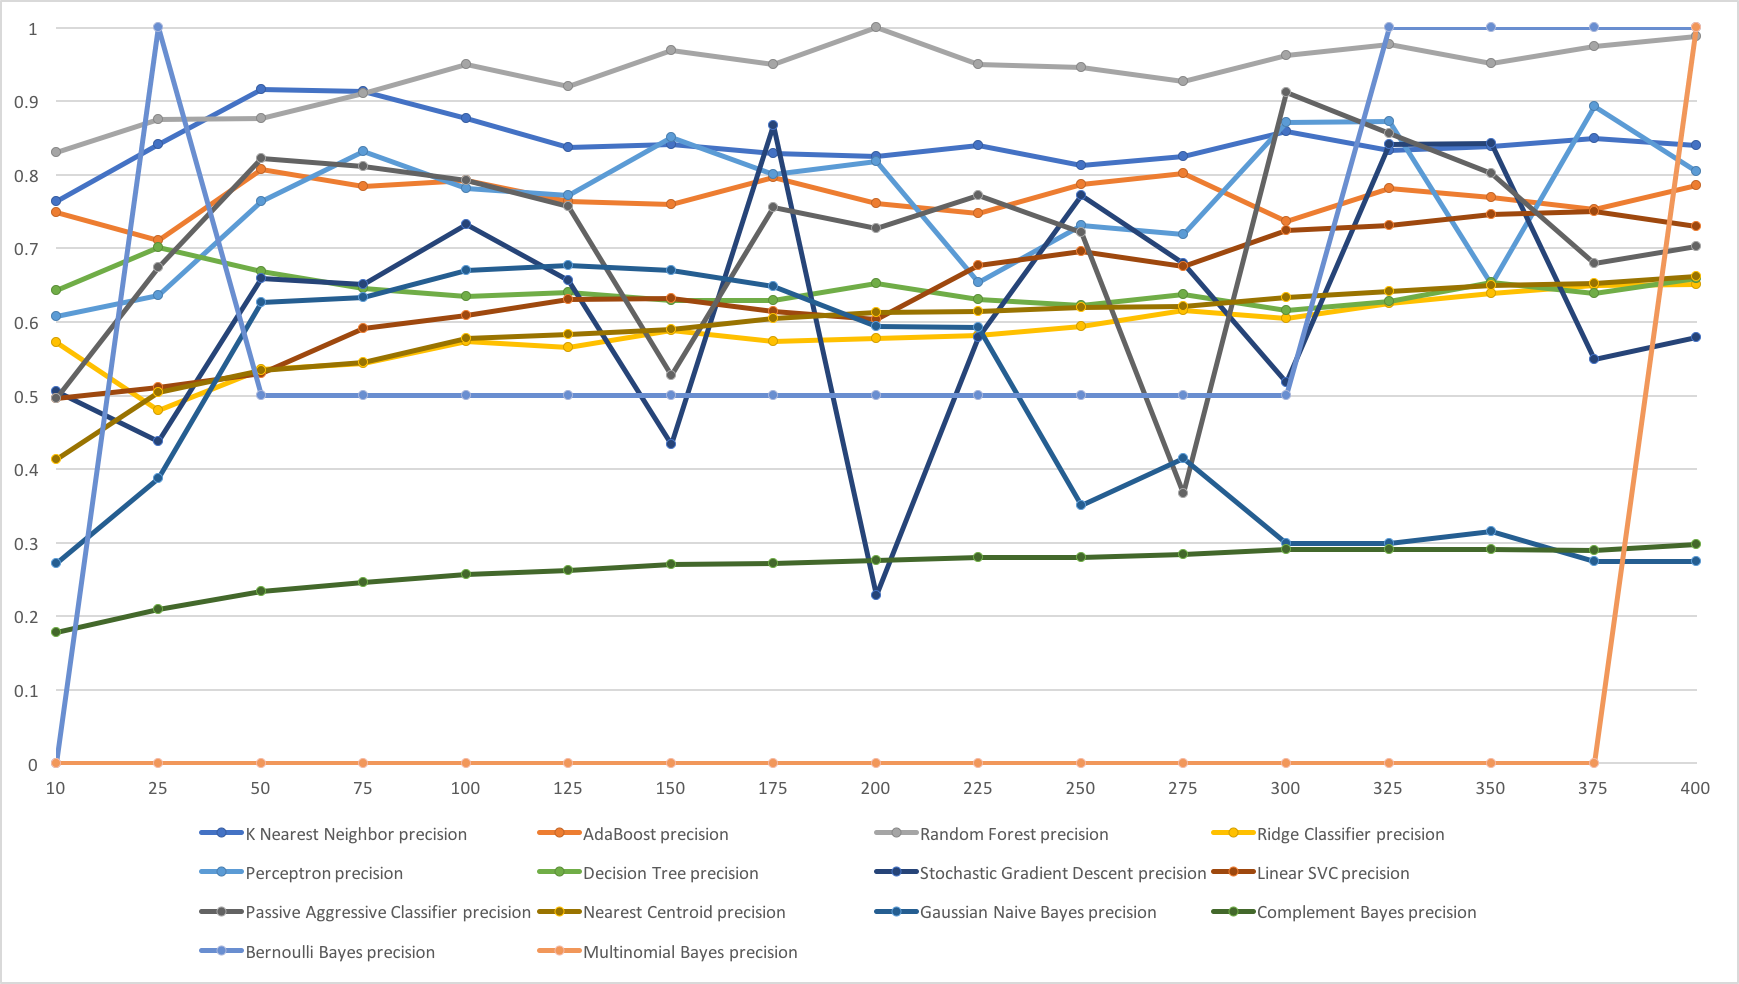
\includegraphics[width=0.8\columnwidth,keepaspectratio]{img/bow-pre.png}
	\caption{Grafik des Precision-Verlaufs bei Bag of Words}
\end{figure}
\subsubsection{Binäres Bag of Words}
Bei der Methode \glqq binäres Bag of Words\grqq{} können mehrere Algorithmen einen F1-Score nahe der 0.8 Grenze verbuchen.
Der beste Algorithmus ist Perceptron, welcher mit 325 Features einen F1-Score von 0.8 verzeichnet.\\
Der SGDClassifier erreicht ebenfalls einen F1-Score von 0.8, jedoch mit einer höheren Anzahl von Features.
Dies bedeutet das SGDClasifier potenziell länger für die Feature-Extraction benötigt und somit ist Perceptron der favorisierende Algorithmus bei dieser Variante.\\
\begin{figure}[H]	
	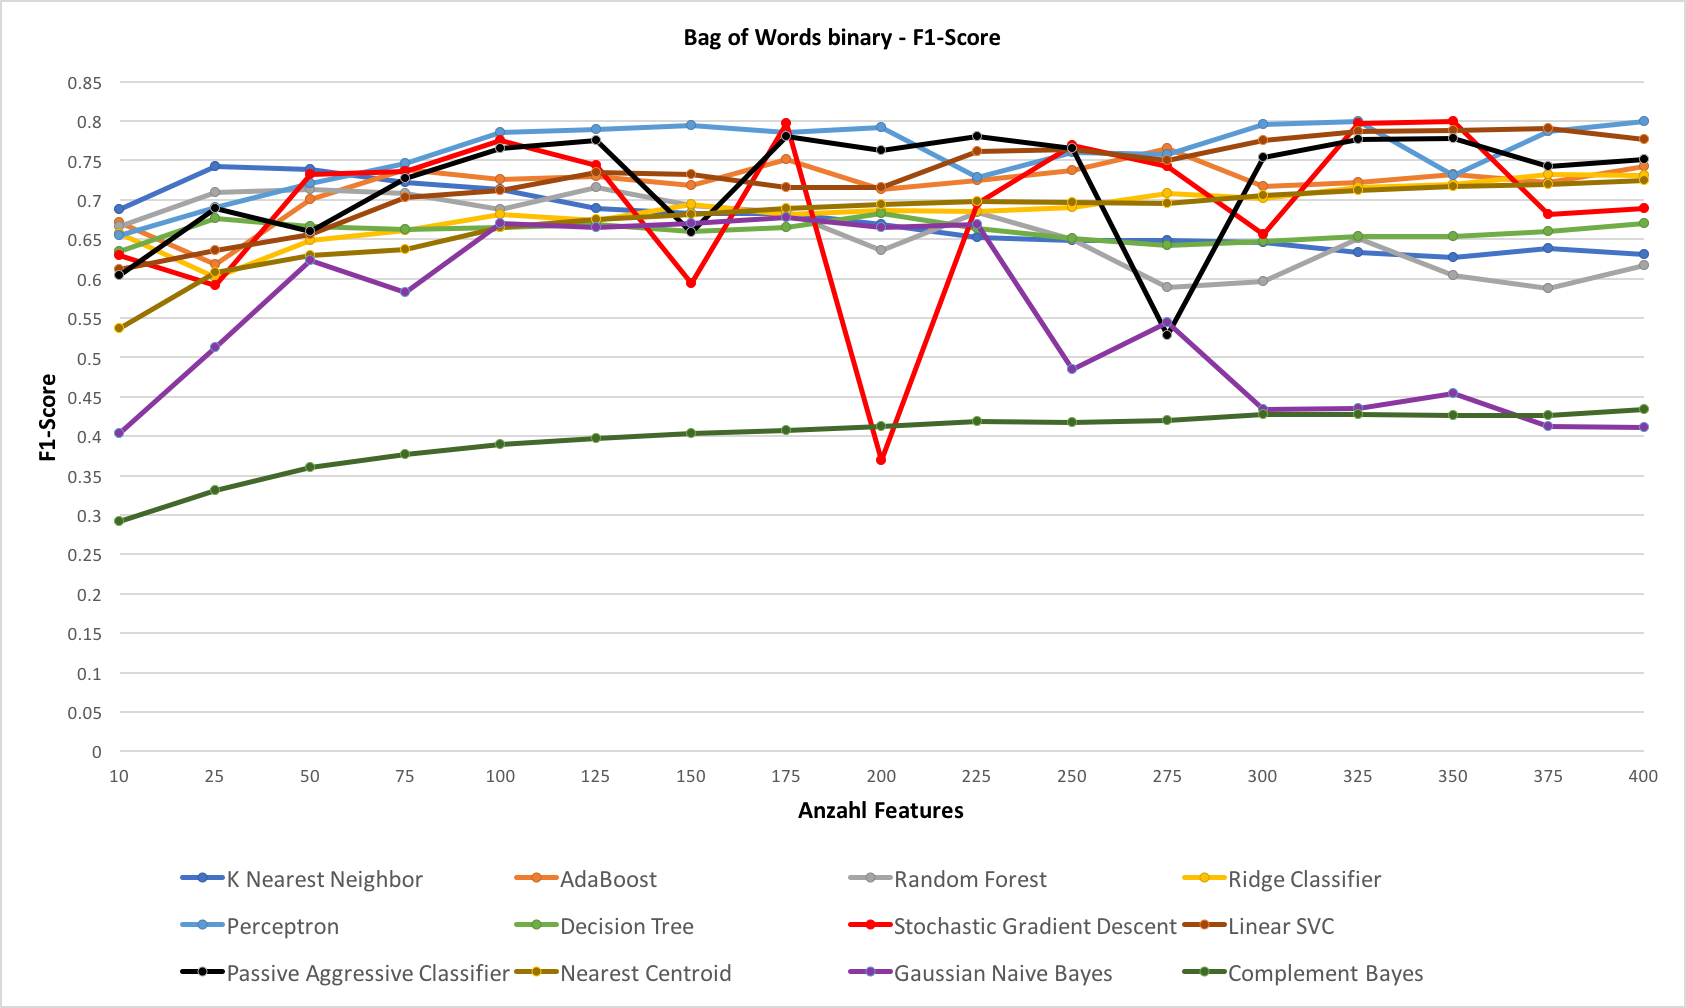
\includegraphics[width=0.8\columnwidth,keepaspectratio]{img/bow-bin-f1.png}
	\caption{Grafik des F1-Score-Verlaufs bei binärem Bag of Words}
\end{figure}
Bei der Precision ist der RandomForest Algorithmus ebenfalls die beste Wahl.
Er erreicht wieder die höchsten Prcecision-Werte bei einer vernünftigen Anzahl Features.\\
Ebenfalls springt der Bernoulli-Bayes wieder zwischen 1.0 und 0.5 umher.
Bei dieser Variante wird der Bernoulli-Bayes als keine Alternative gegenüber dem RandomForest in Betracht gezogen.
\begin{figure}[H]	
	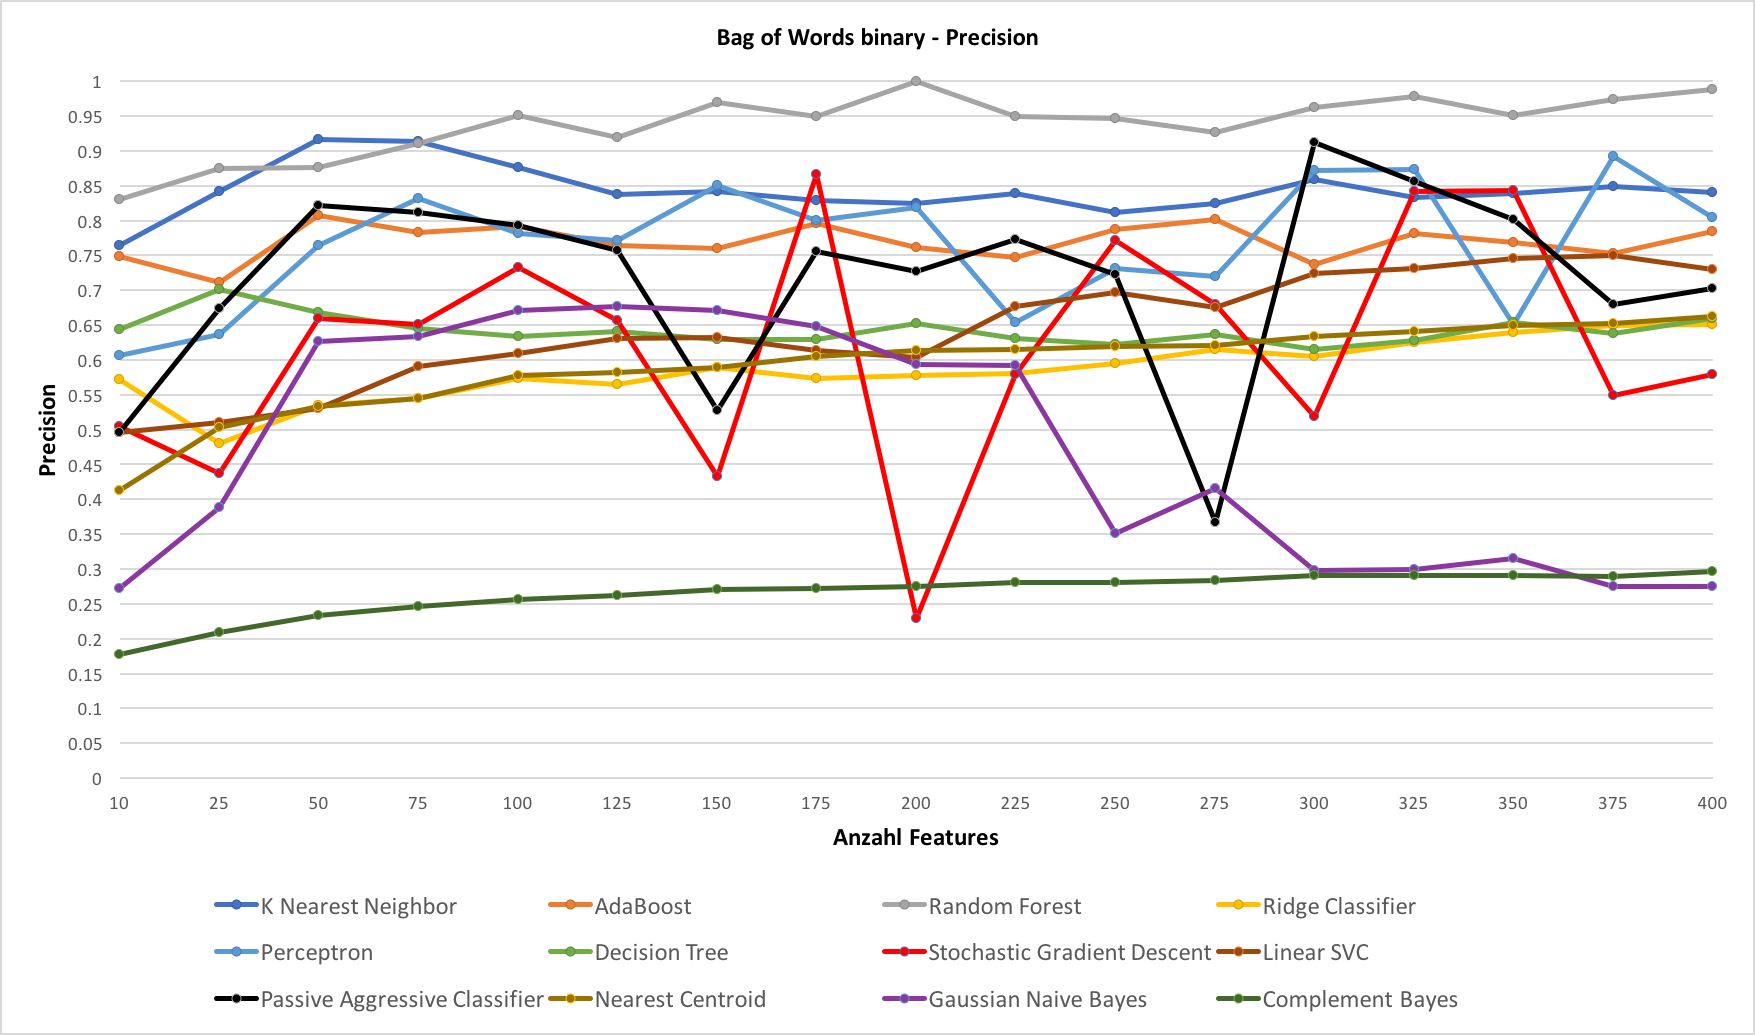
\includegraphics[width=0.8\columnwidth,keepaspectratio]{img/bow-bin-pre.png}
	\caption{Grafik des Precision-Verlaufs bei binärem Bag of Words}
\end{figure}
\subsubsection{TF-IDF}
Bei der Verwendung von TF-IDF sind mehrere Algorithmen mit ihren F1-Scores im Bereich 0.7 bis 0.8.
Der SGDClassifier Algorithmus kann als einziger die Grenze von 0.8 durchbrechen und ist somit der Algorithmus mit dem besten F1-Score.\\
\begin{figure}[H]	
	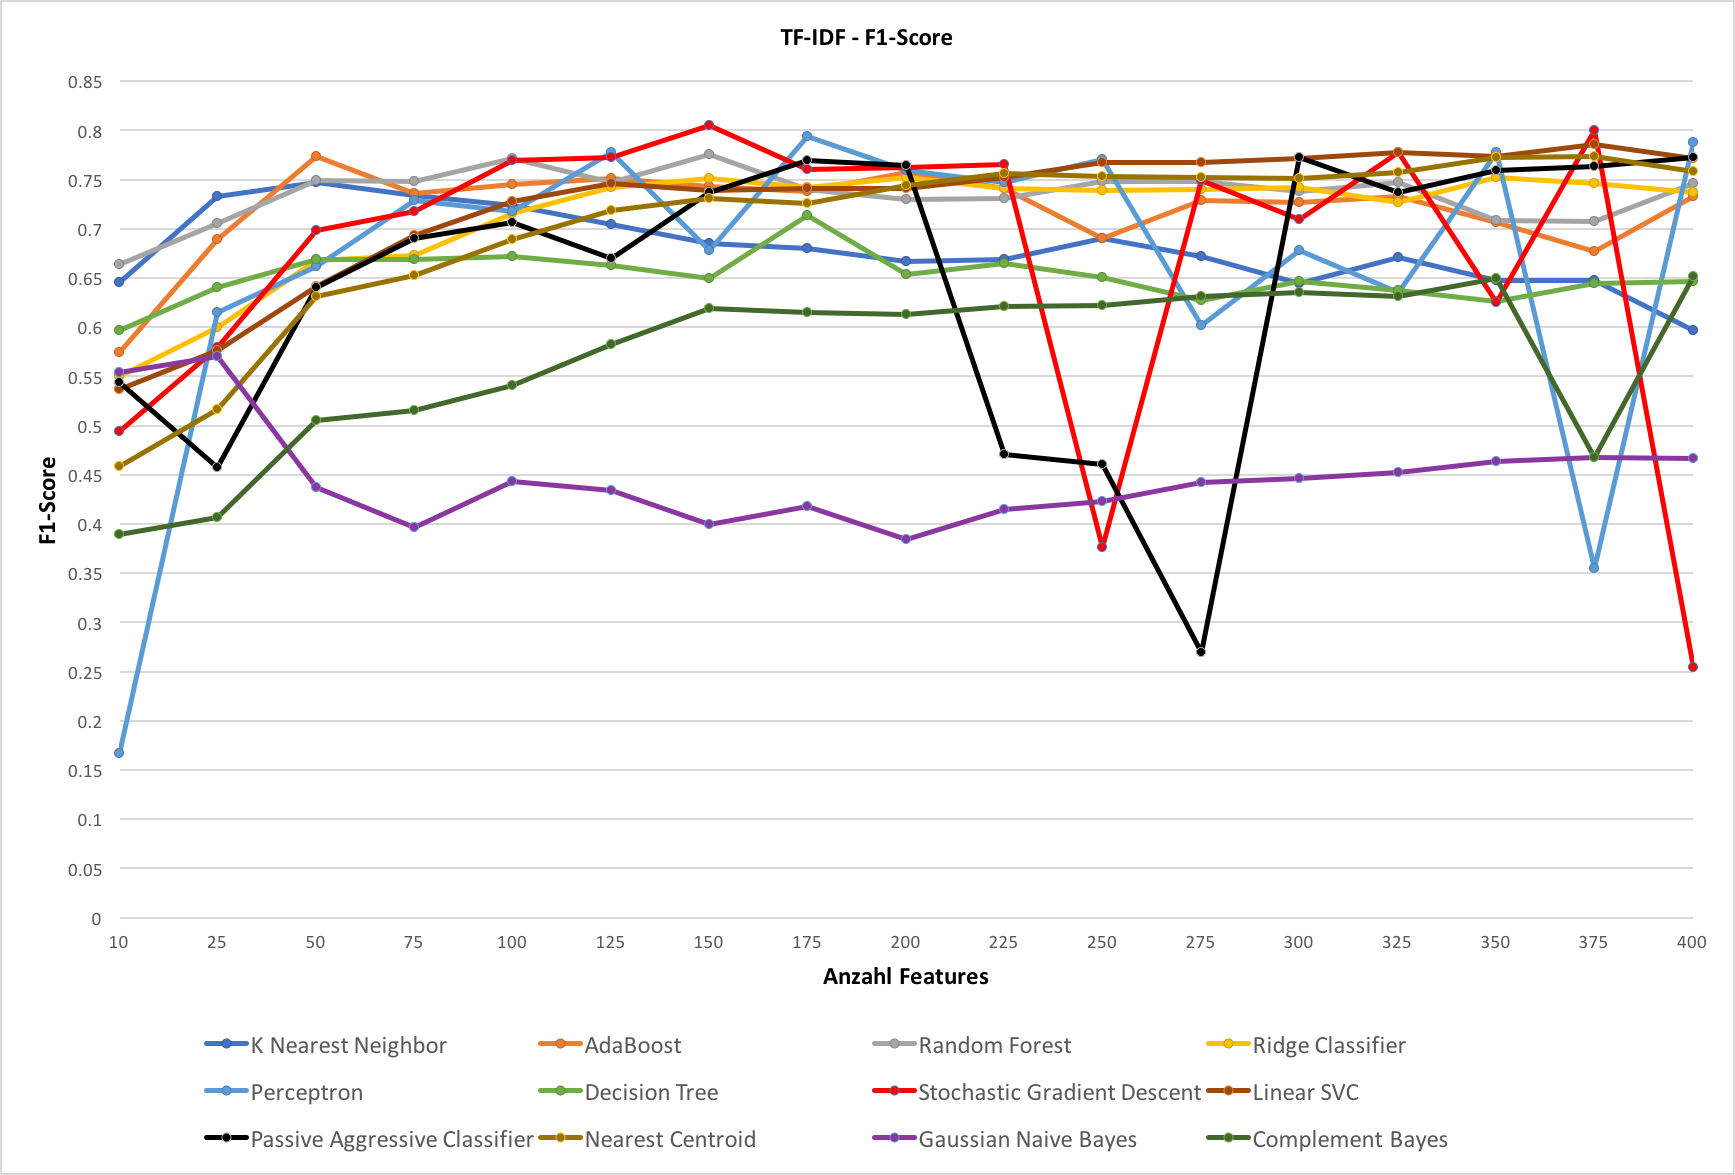
\includegraphics[width=0.8\columnwidth,keepaspectratio]{img/tfidf-f1.png}
	\caption{Grafik des F1-Score-Verlaufs bei TF-IDF}
\end{figure}
Bei der Precision ist der RandomForest Algorithmus ebenfalls wieder der Spitzenreiter.
Er erzielt bei fast jeder Anzahl von Features die beste Precision und kann bei 325 Features sein Maximum erreichen.
\begin{figure}[H]	
	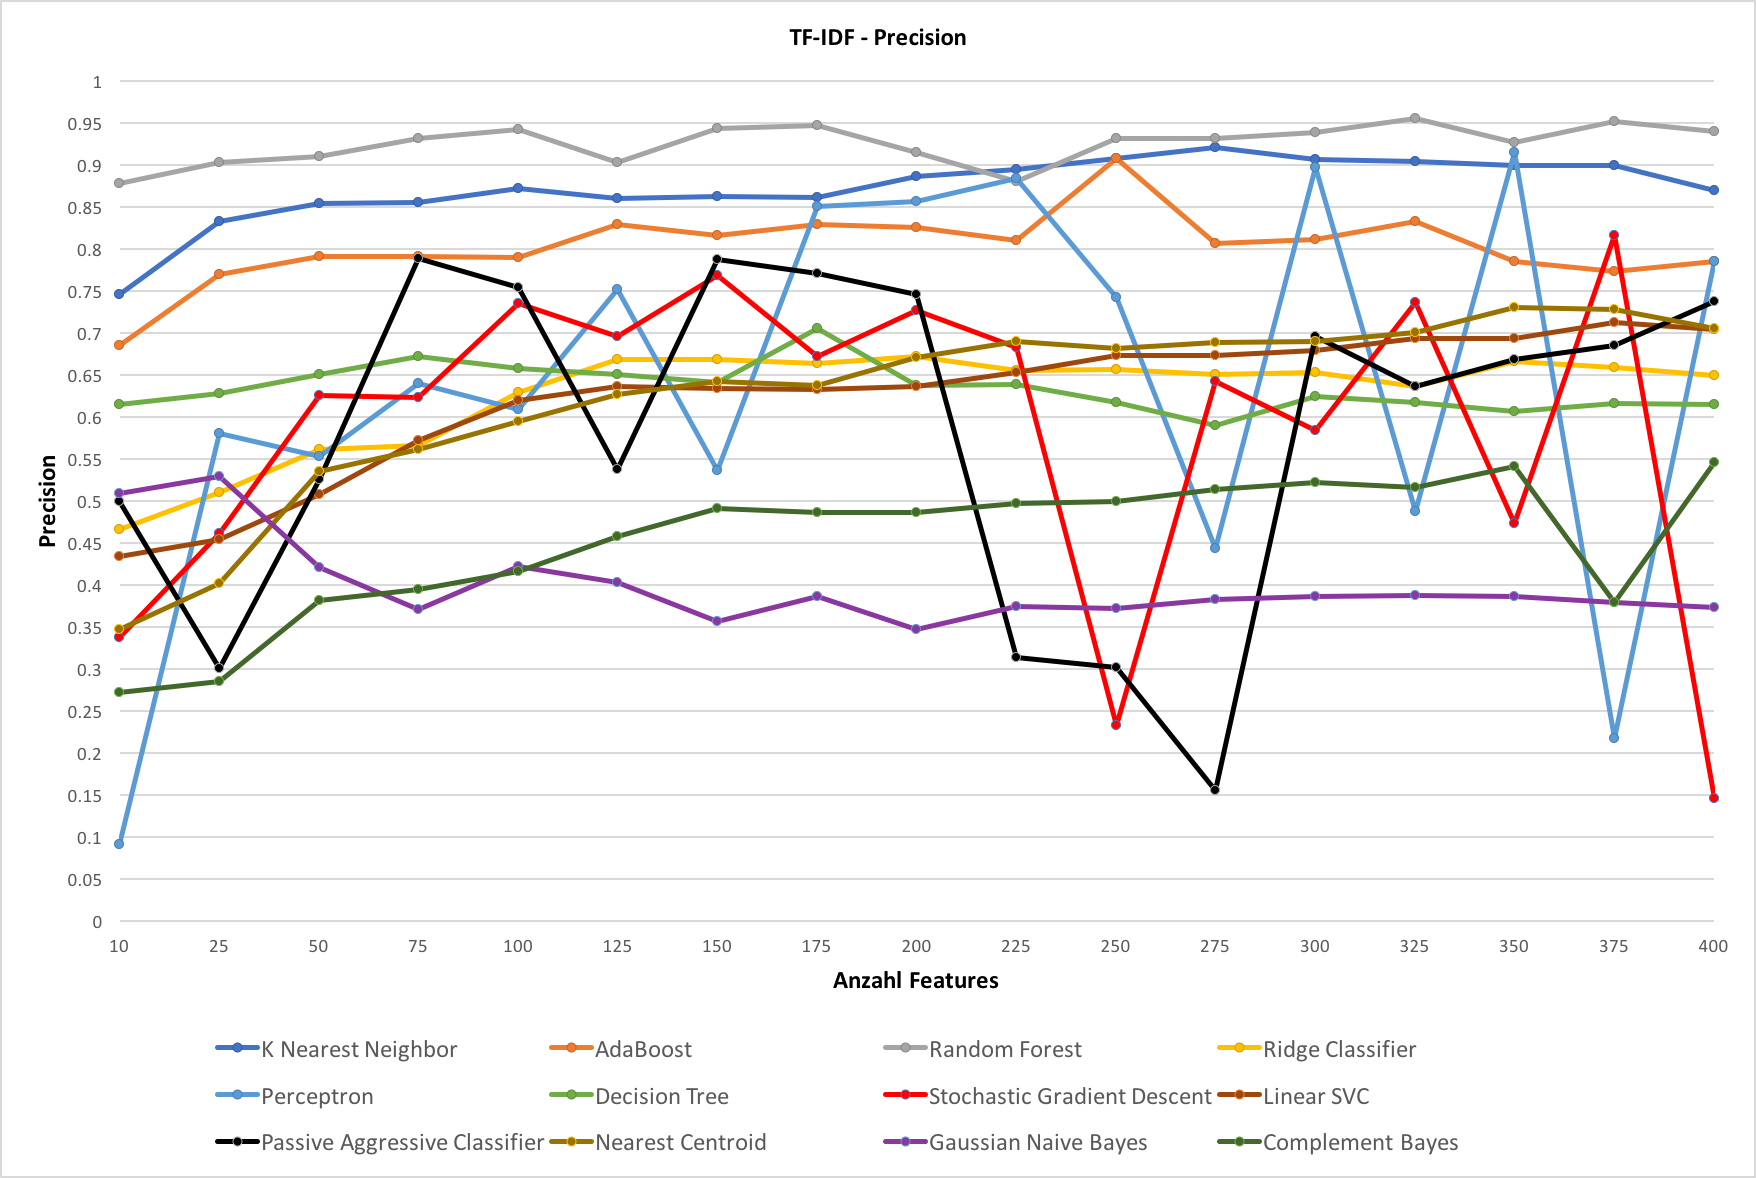
\includegraphics[width=0.8\columnwidth,keepaspectratio]{img/tfidf-pre.png}
	\caption{Grafik des Precision-Verlaufs bei TF-IDF}
\end{figure}
\subsection{Hyperparametertuning}
Die sechs Modelle, welche aus dem vorherigen Experiment, als die besten entnommen wurden, werden mittels Kreuzvalidierung auf optimale Hyperparameter durchsucht.
\subsubsection{Modelle mit bestem F1-Score}
Die drei Modelle AdaBoost, SGDClassifier und Perceptron können die besten F1-Scores erzielen.\\
\begin{table}[H]
	\caption{Auwertung Hyperparametertuning für AdaBoost mit binärem Bag of Words}
	\centering
	\begin{tabular}{|l|l|l|l|}
		\hline
		 & F1-Score & Precision & Recall\\
		\hline
		Vor Hyperparametertuning & 0.778 & 0.837 & 0.727 \\
		Nach Hyperparametertuning & 0.788 & 0.817 & 0.761 \\
		\hline
	\end{tabular}
\end{table}
\begin{table}[H]
	\caption{Auwertung Hyperparametertuning für Perceptron mit Bag of Words}
	\centering
	\begin{tabular}{|l|l|l|l|}
		\hline
		& F1-Score & Precision & Recall\\
		\hline
		Vor Hyperparametertuning & 0.8 & 0.872 & 0.739 \\
		Nach Hyperparametertuning & 0.579 & 0.426 & 0.903 \\
		\hline
	\end{tabular}
\end{table}
\begin{table}[H]
	\caption{Auwertung Hyperparametertuning für SGDClassifier mit TF-IDF}
	\centering
	\begin{tabular}{|l|l|l|l|}
		\hline
		& F1-Score & Precision & Recall\\
		\hline
		Vor Hyperparametertuning & 0.805 & 0.768 & 0.847 \\
		Nach Hyperparametertuning & 0.762 & 0.682 & 0.864 \\
		\hline
	\end{tabular}
\end{table}
Auffällig ist, dass AdaBoost als einziges Modell bessere Hyperparameter mittels Hyperparemtertuning finden konnte.\\
AdaBoost kann seinen Recall verbessern und gleichzeitig verschlechtert sich seine Precision.
Da die Recallsteigerung grösser als der Precisionabfall ist, wird der F1-Score nach oben korrigiert.\\
Die anderen beiden Modelle erzielen mit den neuen Parametern schlechtere Werte.
Beide können den Recall verbessern, jedoch müssen sie massive Gefälle bei der Precision einbüssen.
Da die Precision viel stärker abgenommen, als der Recall zugenommen hat, wird der F1-Score schlechter.\\
Perceptron hat im Vergleich zum SGDClassifier einen leicht tieferen F1-Score, jedoch ist seine Precision deutlich höher.
Da für den schlussendlichen \glqq Use-Case\grqq{} Precision wichtig ist, wird das Perceptron-Modell für weitere Auswertungen verwendet.
\subsubsection{Modelle mit bester Precision}
Das Modell RandomForest kann für alle drei Feature-Extraction Methoden jeweils den besten Precision-Score erzielen.\\
\begin{table}[H]
	\caption{Auwertung Hyperparametertuning für RandomForest mit binärem Bag of Words}
	\centering
	\begin{tabular}{|l|l|l|l|}
		\hline
		& F1-Score & Precision & Recall\\
		\hline
		Vor Hyperparametertuning & 0.636 & 1.0 & 0.466 \\
		Nach Hyperparametertuning & 0.736 & 0.8 & 0.682 \\
		\hline
	\end{tabular}
\end{table}
\begin{table}[H]
	\caption{Auwertung Hyperparametertuning für RandomForest mit Bag of Words}
	\centering
	\begin{tabular}{|l|l|l|l|}
		\hline
		& F1-Score & Precision & Recall\\
		\hline
		Vor Hyperparametertuning & 0.636 & 1.0 & 0.466 \\
		Nach Hyperparametertuning & 0.768 & 0.829 & 0.716 \\
		\hline
	\end{tabular}
\end{table}
\begin{table}[H]
	\caption{Auwertung Hyperparametertuning für RandomForest mit TF-IDF}
	\centering
	\begin{tabular}{|l|l|l|l|}
		\hline
		& F1-Score & Precision & Recall\\
		\hline
		Vor Hyperparametertuning & 0.747 & 0.956 & 0.614 \\
		Nach Hyperparametertuning & 0.794 & 0.823 & 0.767 \\
		\hline
	\end{tabular}
\end{table}
Alle drei Varianten können ihren F1-Score verbessern.
Die Verbesserung erfolgt nur im Bereich Recall, welcher initial bei allen drei Modellen relativ tief war.
Zusätzlich sinken bei allen drei Modellen die Precision-Scores.
Bei beiden Varianten mit Bag of Words, waren alle drei initialen Scores identisch und die Precision maximal.\\
Da in diesem Abschnitt auf die beste Precision geachtet wird, ist das Modell mit binärem Bag of Words und mit den Standardparametern die beste Variante.
\newpage

\chapter{Komponenten}
\section{Webcrawler}
\subsection{Beschreibung der Technologie}
\subsubsection{Apache Storm}
StormCrawler basiert auf Apache Storm, einem Opensource Framework zur verteilten Stream-Verarbeitung.
Die Architektur von Apache Storm basiert auf den folgenden Komponenten:
\begin{itemize}
	\item Spout - Komponente zum Einlesen von Daten-Streams
	\item Bolt - Komponente zum Verarbeiten von Daten-Streams
	\item Tupel - Datensatz, welcher zwischen den Komponenten weitergegeben wird
	\item Topologie - Ein Netz bestehend aus Spouts und Bolts
\end{itemize}
Jede Komponente ist als eigene Java-Klasse definiert und beinhaltet zwingend die folgenden Methoden:
\begin{itemize}
	\item declareOutputFields() - Definition des Ausgabeschemas des Tupels
\end{itemize}
Jeder Bolt enthält zudem eine weitere Methode:
\begin{itemize}
	\item execute() - Ausführen des Tasks der Komponente
\end{itemize}
In einer Topologie werden verschiedene Spouts und Bolts miteinander verknüpft, um einen Prozess durchzuführen, wie in \cref{fig:topology} gezeigt wird.
\begin{figure}[H]	
	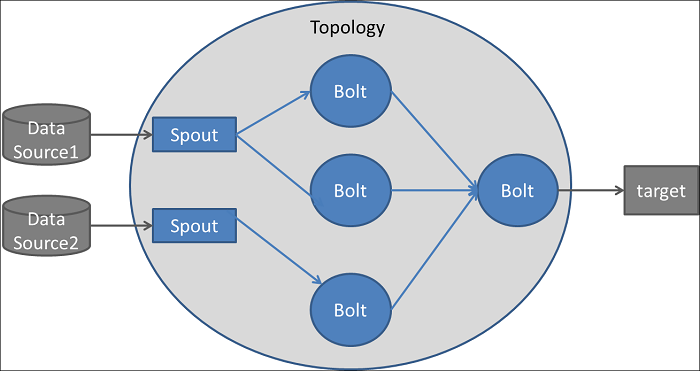
\includegraphics[width=0.8\columnwidth,keepaspectratio]{img/storm-topology.png}
	\caption{Beispieltopologie\\ Quelle: https://dzone.com/articles/apache-storm-architecture}
	\label{fig:topology}
\end{figure}
Dabei hat der Spout die Aufgabe, Daten aus einer Quelle (z.B. Datei, Datenbank, Array) einzulesen und daraus ein Tupel zu bilden.
Dieses Tupel wird an die weiteren Bolts der Topologie weitergegeben und von diesen verarbeitet.
Diese Verarbeitung muss nicht seriell stattfinden, die Topologie kann auch Gabelungen beinhalten, die dementsprechend Bolts benötigen, welche entscheiden, an welchen Folge-Bolt das Tupel weitergegeben werden soll.
Zudem ist eine Webapplikation verfügbar, die eine Übersicht über die Informationen wie eine Topologieübersicht, der Status der jeweiligen Komponenten sowie Fehlermeldungen anzeigt.
\subsubsection{StormCrawler SDK}
StormCrawler ist ein Opensource Software Development Kit, welches auf Apache Storm aufbaut und in Java entwickelt wurde.
Er dient als Baukasten, um einen Webcrawler aufzubauen, der skalierbar, stabil und sehr effizient ist.
Er beinhaltet verschiedene Spouts und Bolts, die explizit zum Crawlen von Websites vorgefertigt wurden.
Zudem berücksichtigt er die Regeln des Webcrawlings, also Meta-Tags oder Robot.txt Dateien, welche deklarieren, ob eine Website gecrawlt werden darf.
Weiter ist er so eingerichtet, dass Webpages derselben Website mit einer Zeitverzögerung abfragt, damit diese nicht überlastet werden.
StromCrawler ist standardmässig so eingerichtet, dass nur Webpages desselben Hosts gecrawlt werden.
\subsubsection{Docker}
Docker besitzt verschiedene Bedeutungen. 
Docker kann sich auf den Namen der Firma Docker Inc."fussnote" beziehen oder auf die eigentliche Software.
In diesem Kontext wird Docker als die Software zum Erstellen von Linux-Containern verwendet.
Mithilfe von Docker können ressourcenarme, modulare virtuelle Maschinen erstellt werden, welche auch Container genannt werden.
Diese Container können dann einfach kopiert, ersetzt oder auf einem anderen System verwendet werden.
\footnote{\url{https://www.redhat.com/de/topics/containers/what-is-docker}}
Linux-Container verwenden den Linux-Kernel und seine Funktionen, einzelne Prozesse isolieren zu können.
Der Vorteil von Containern ist, dass alle Abhängigkeiten mit der ausführbaren Software in den Container gepackt werden können und somit jede Umgebung, die den gleichen Container verwendet, auch den gleichen Softwarestand besitzt.
Docker Container werden mit einem einzigen Konfigurationsfile beschrieben.
Dieses Konfigurationsfile, das sogenannte Dockerfile, definiert alle Notwendigkeiten, um den Docker Container zu realisieren.
Im Dockerfile werden Instruktionen für das Erstellen des Images definiert.
Da Dockerfiles einfache Textdateien sind, können sie, wie jeder andere Sourcecode, mit Git, SVN oder anderen Versionsverwaltungen verwaltet werden.
Aus Dockerfiles werden Docker Images erstellt.
Durch Dockerfiles können Docker Images erstellt werden, welche wiederum den dadurch definierten Container erstellen und starten.
Grundsätzlich kann das Docker Image mit einer Klasse im Objekt-Orientierten-Programmieren verglichen werden und der Docker Container wäre eine laufende Instanz der entsprechenden Klasse. 
%\footnote{\url{https://stackoverflow.com/questions/3175105/inserting-code-in-this-latex-document-with-indentation}}

\subsubsection{Docker-Compose}
Mit Docker Containern können auch Micro-Services Architekturen realisiert werden, wodurch jeder Container einen eigenen Service darstellt.
Das manuelle Starten jedes einzelnen Containers erweist sich jedoch als ineffizient, deswegen übernimmt die Software "Docker-Compose" diese Aufgabe.
Mithilfe von Docker-Compose können mehrere Docker Container verknüpft und gleichzeitig gestartet werden.
Die Abhängigkeiten zwischen den Containern wird ebenfalls mit einem Konfigurationsfile, dem Composefile, definiert.
Wahlweise können Dateiordner vom Hostsystem in einzelne Container angehängt werden, damit die Container Daten dort abspeichern oder abrufen können.
Dies ist insofern wichtig, da sobald die Container gestoppt werden, all ihre internen Daten verloren gehen.
Die Containerinhalte existieren nur so lange, wie auch die Container existieren.
Docker-Compose erstellt für alle Container in einer Gruppierung einzigartige ID-Namen, damit alle Container innerhalb der Gruppierung miteinander kommunizieren können.
\footnote{\url{https://github.com/DigitalPebble/storm-crawler/}}
\subsection{Konfiguration des StormCrawlers}
Die Grundlage der Konfiguration ist die Standardtopologie des Stromcrawlers auf Github.
\footnote{\url{https://docs.docker.com/develop/develop-images/dockerfile_best-practices/}}
Diese besteht aus den folgenden Komponenten und geht wie folgt vor:
\begin{enumerate}
	\item MemorySpout - Einlesen einer URL aus einem Array
	\item URLPartitionerBolt - Geneneriert einen eindeutigen Partition Key
	\item FetcherBolt - Ruft die Webpage ab
	\item SiteMapParserBolt - Erkennt die Sitemap-Datei und fügt weitere URLs zum MemorySpout hinzu
	\item FeedParserBolt - Extrahiert URLs aus Feeds
	\item JSoupParserBolt - Extrahiert Informationen wie Metatags oder den Text aus der Webpage
	\item SdtOutIndexer - Gibt die Informationen einer Webpage über die Konsole aus
\end{enumerate}
Ein selbst erstellter Bolt, welcher für das Schreiben des Outputs zuständig ist hat in dieser Konfiguration den StdOutIndexer ersetzt.
Dieser schreibt für jede Webpage, die erreichbar ist und gecrawlt werden darf, eine JSON Datei mit den folgenden Informationen:
\begin{itemize}
	\item \glqq date \grqq  - Zeitpunkt, zu welchem die Webpage aufgerufen wurde
	\item \glqq text \grqq  - Vom Webcrawler extrahierter Text, welcher die Webpage beinhaltet
	\item \glqq encoding \grqq  - Das von der Webpage verwendete Encoding
	\item \glqq title \grqq  - Inhalt des gleichnamigen HTML-Metatags
	\item \glqq url \grqq  - URL der Webpage
	\item \glqq content \grqq  - Der statische HTML-Inhalt der Webpage	
\end{itemize}
Der Dateiname dieser JSON Dateien wird aus der URL der Webpage generiert. 
Sonderzeichen, die in Dateinamen nicht erlaubt sind, werden entfernt. Falls die URL länger ist, als die erlaubte Dateinamenslänge, wird diese abgeschnitten und mit einem zufälligen vierstelligen Suffix erweitert.
Zudem kommt darin eine Spracherkennung \glqq Lingua\footnote{\url{https://github.com/pemistahl/lingua}}\grqq{} zum Einsatz, welche anhand des Textes einer Webpage detektiert, ob sie mehrheitlich in deutsch geschrieben wurde.
Als deutsch detektierte Webpages werden in einen separaten Output-Ordner gespeichert, damit diese nachfolgend von Hand gelabelt werden können.
Trotzdem ist es wichtig, dass alle aufgerufenen Webpages gespeichert werden, damit im Anschluss des Crawlens eine Aussage gemacht werden kann, wie viele Einträge des Seeds effektiv gecrawlt wurden.

\section{Klassifizierung}
\subsection{Verwendete Technologien}
\subsubsection{Luigi}
Luigi ist ein Pipelining-Tool, welches von Spotify entwickelt und später als Open-Source Projekt veröffentlicht worden ist.
Pipelining dient dazu, mehrere Tasks miteinander zu verknüpfen, das Ausführen zu Automatisieren und somit eine grössere Aufgabe zu verrichten.
Pipelining wird meist im Kontext von Big Data oder Machine-Learning angewendet, wo sich viele einzelne Tasks mit grossen Datenmenge beschäftigen.
Luigi wird selbst von Spotify in der Produktion verwendet und bietet unter anderem folgende Features:
\begin{itemize}
	\item Einzelne Tasks idempotent ausführen
	\item Teilschritte oder gesamte Pipeline kann über Konsolenausgabe oder Webinterface überwacht werden
	\item Fehlerfälle können protokolliert werden und dementsprechend reagiert werden
	\item Abhängigkeiten von Tasks werden selbstständig von Luigi gelöst
	\item Luigi ist komplett in Python aufgebaut und kann auch mit Python konfiguriert werden
\end{itemize}
Die einzelnen Tasks werden mit Python-Klassen realisiert.
Luigi ist so aufgebaut, dass jeder Task ein Input-File liest, von dem die Ausgabe des vorherigen Tasks eingelesen wird und ein Output-File schreibt, welches als Input-File des anschliessenden Tasks benutzt wird.
Dadurch kann Luigi die Zustände der einzelnen Tasks überwachen und bei einem Fehlerfall die Pipeline dort wieder starten, wo sie sich aufgehängt hat.
Damit Luigi die Abhängigkeiten und das Überwachen bewerkstelligen kann, benötigt jede Klasse in der Pipeline folgende 3 Funktionen:
\begin{itemize}
	\item Funktion requires(), Angabe auf welche Tasks Abhängigkeiten bestehen
	\item Funktion run(), Bereich, wo die eigentliche Logik des Tasks ist
	\item Funktion output(), wohin die Ausgabe geschrieben wird
\end{itemize}
In dieser Arbeit wurde Luigi verwendet, um die Klassifizierung zu verknüpfen.
Es wurden zwei verschiedene Arten von Pipelines erstellt.
Die Entwicklungspipeline diente zur Entwicklung der Regeln/Machine-Learning-Modelle für die Klassifizierung.
Die Klassifizierung beinhaltet das Lesen der gecrawlten Daten, das Preprocessing, das Klassifizieren und das Evaluieren der Klassifizierung.
Die daraus folgende Pipeline beinhaltet folgende Tasks:
\begin{itemize}
	\item Importer, import die gecrawlten Websites und speichert sie in einer CSV-Datei
	\item Preprocessor, wendet übliche Preprocessing-Schritte an den Daten an
	\item RuleBasedClassifier, regelbasierte Klassifizierung der Daten 
	\item MLClassifier, Klassifizierung der Daten mittels Machine-Learning
	\item Evaluator, Auswertung der Klassifizierung von Daten (Nur im Entwicklunsmodus)
\end{itemize}
\subsubsection{Scikit Learn}
Scikit Learn ist eine freie Programmierbibliothek für Python, mit welcher man effizient Projekte für Data-Mining, Datenvisualisierung und Machine-Learning erarbeiten kann.
Scikit Learn ist unter BSD lizenziert und für den kommerziellen Nutzen frei verfügbar.
Sie ist eine der bekanntesten Standardbibliotheken für Machine-Learning, wird unter anderem von grossen Namen wie Google finanziell unterstützt und besitzt eine rege Contribution-Community auf Github\footnote{\url{https://github.com/scikit-learn/scikit-learn}}.\\
Scikit Learns Stärken liegen in den Machine-Learning Bereichen \glqq Supervised Learning\grqq{} und \glqq Unsupervised Learning\grqq{}.
Die API von Scikit Learn bietet eine Vielzahl von Algorithmen für Klassifizierung, Regression, Clustering, Dimensionsreduktion, Modelselektion und Preprocessing an und deckt somit die ganze Machine-Learning Pipeline ab.
Scikit Learn bietet für fast jeden Algorithmus oder Technik in der API eine Beispielimplementation an, welche für Fast-Prototyping  als Fundament übernommen werden kann.
\subsection{Preprocessing}\label{preprocessing}
Das Preprocessing wurde entwickelt, um den Inhalt des Dokuments auf eine standardisierte Form zu bringen.
Die folgenden Methoden können sowohl auf den Text eines Dokuments sowie auch auf den Titel angewendet werden.
Diese werden sequenziell in der unten aufgeführten Reihenfolge angewandt und können mittels Konfiguration sowohl für den Text als auch Titel eines Dokuments ein- oder ausgeschaltet werden.
\subsubsection{Gross-/Kleinschreibung}
Alle Buchstaben, welche grossgeschrieben sind, werden durch die entsprechenden Kleinbuchstaben ersetzt.
\subsubsection{Umlaute ersetzen}
Umlaute werden durch ihre verwandten Selbstlaute ersetzt, genauer:
\begin{itemize}
	\item ä $\rightarrow$ a
	\item ö $\rightarrow$ o
	\item ü $\rightarrow$ u
\end{itemize} 
\subsubsection{Preisdetektor}
Da Menüs häufig in Verbindung mit Preisen vorkommen und in weiteren Preprocessing-Schritten Zahlen und Sonderzeichen entfernt werden, ist es von Vorteil, diese Informationen nicht zu verlieren.
Daher erkennt diese Methode verschiedene Varianten von Preisen mittels Regulären Ausdrücken (Regex, Regular Expression) und ersetzt diese mit einem Schlüsselwort.
% Varianten genauer ausführen
Die folgenden Varianten von Preisen wird erkannt:
\begin{itemize}
	\item preisangabe + chf/fr/sfr
	\item preisangabe
	\item chf/fr/sfr + preisangabe
\end{itemize} 
Zudem wird zwischen unterschieden, wie viele Stellen der Preis hat.
Die nun aufgeführte Liste zeigt die verschiedenen Schlüsselwörter:
\begin{itemize}
	\item Einstellig $\rightarrow$ onedigitprice
	\item Zweistellig $\rightarrow$ twodigitprice
	\item Dreistellig $\rightarrow$ threedigitprice
\end{itemize} 
Um Zeitangaben nicht als Preise zu erkennen, werden bei Preisangaben ohne Währungsangabe nur Beträge mit Rappenbeträgen, welche 60 oder höher sind, erkannt.
\subsubsection{Sonderzeichen entfernen}
Alle Sonderzeichen, die nicht in der folgenden Auflistung vorkommen, werden durch einen Leerschlag ersetzt:
%Eventuell noch anpassen, da Grossbuchstaben nicht mehr relevant sind (EVTL. é usw auch noch ersetzen?)
\begin{itemize}
	\item éàèÉÀÈäöüÄÖÜa-zA-Z
\end{itemize} 
\subsubsection{Einzelne Zeichen entfernen}
Jedes einzelne Zeichen, also solche, die sowohl vorne als auch hinten an einen Leerschlag angrenzen, werden entfernt.
\subsubsection{Multiple Leerschläge entfernen}
Da durch die vorhergehenden Schritte oft multiple Leerschläge anfallen, werden diese auf einen Leerschlag reduziert.
\subsubsection{Stammformreduktion}
Dieses Verfahren führt verschiedene morphologische Varianten eines Wortes auf ihren gemeinsamen Stamm zurück.
Dafür wird der Stemmer \glqq Cistem\footnote{\url{https://github.com/LeonieWeissweiler/CISTEM}}\grqq{} verwendet, da für die deutsche Sprache nur wenig Alternativen vorhanden sind. 
\subsubsection{Getränkedetektor}
% Referenz Cistem
Eine Liste mit Einträgen diverser Getränke bildet die Grundlage dieser Methode.
Wenn im Text ein Getränk dieser Liste vorhanden ist, wird es durch das Schlüsselwort \glqq beverageentity\grqq{} ersetzt.
Damit soll erreicht werden, dass ein einheitliches Merkmal geschaffen wird.
\subsubsection{Stoppwörter entfernen}
Bei Stoppwörter handelt es sich um Wörter, welche keine Relevanz für den Inhalt eines Texts haben, aber oft vorkommen.
Eine Stoppwortliste führt 1720 solcher Wörter in deutsch auf. Sie ist aus mehreren Quellen zusammengesetzt worden.
% Quellen Stoppwortliste aufführen?
Wenn eines dieser Wörter im Text vorkommt, wird es entfernt.
\subsection{Regelbasierte Klassifizierung}
Verschiedene Algorithmen kommen beim regelbasierten Klassifizieren zum Einsatz, welche nun genauer erläutert werden.
\subsubsection{Menü im Titel}
Dieser simple Algorithmus kontrolliert, ob das Wort \glqq menu\grqq{} im Metatag \glqq Title\grqq{} vorkommt.
Falls ja, wird das Dokument als Menüseite klassiert.
\subsubsection{Preisdetektor}
Dieser Algorithmus funktioniert dankt der Preprocessing-Methode, welche den Preis erkennt.
Sofern ein zweistelliger Preis im Text erkannt wurde, wird das Dokument als Menüseite klassifiziert. Dies unter der Annahme, dass Menüpreise oft zweistellig sind, im Gegensatz zu Getränkepreisen welche häufig einstellig sind und Hotelpreisen, die meist dreistellig sind.
Die Anzahl vorhandener Preise kann über die Konfiguration angegeben werden.
\subsubsection{Kombination aus Menü im Titel und Preisdetektor}
Diese Kombination führt eine sequenzielle Klassifikation aus.
Im ersten Schritt wird der Mechanismus des Algorithmus \glqq Menü im Titel\grqq{} verwendet.
Falls durch diesen keine positive Klassifikation zustande kommt, wird durch den Preisdetektor nochmals neu klassifiziert.
\subsubsection{Listing}
Dieser Algorithmus basiert sowohl auf dem Black- als auch auf dem Whitelisting Ansatz.
Dazu wird eine Blacklist und eine Whitelist verwendet, die von Hand erstellt wurden und Einträge enthalten, welche für die jeweiligen Kategorien typisch sind.
Falls ein Wort einer Liste im Text einer Webpage vorkommt, wird ein Zähler hochgezählt.
Zum Schluss findet eine sequenzielle Klassifizierung statt, das heisst: 
Wenn der Zähler der Blacklist einen konfigurierbaren Schwellwert überschreitet, wird die Webpage als negativ klassifiziert. 
Wenn der Zähler der Whitelist einen konfigurierbaren Schwellwert überschreitet, wird die Webpage als Menüseite klassifiziert.
Falls keiner der beiden Zähler den Schwellwert überschreitet, wird die Webpage ebenfalls als negativ klassifiziert. 
\subsubsection{Bag of Words}
Dieser Algorithmus basiert auf dem statistischen Ansatz namens \glqq Bag of Words\grqq{}.
Dafür wird der komplette Datensatz in einen Trainings- und Testsatz in einem konfigurierbaren Verhältnis aufgeteilt.
Bag of Words zählt für jedes Dokument der Trainingsdaten, wie oft ein Wort darin vorkommt.
In dieser Anwendung wird jedoch nur erkannt, ob ein Wort vorkommt, oder nicht, die Anzahl spielt keine Rolle.
Anhand dieser Wörter wird eine dynamische Black- und Whitelist erstellt, Wörter die in beiden Listen vorkommen, werden entfernt.
Anhand dieser Listen wird der Testdatensatz klassifiziert.
Die Anzahl der Wörter dieser Listen ist konfigurierbar.
Die Klassifikation findet mittels einem Zähler statt.
Für jedes Wort eines Dokuments, welches in der Liste der positiven Beispielen vorkommt, wird der Zähler hochgezählt, für jedes Wort aus der Liste der negativen Beispielen wird er heruntergezählt.
Für die Klassifizierung wird der Zähler mit einem konfigurierbaren Schwellwert verglichen, Falls der Zähler grösser ist als der Schwellwert, wird das Dokument als positiv klassifiziert, ansonsten negativ.
\subsection{Feature-relevante Methoden für Machine-Learning}
\subsubsection{Bag of Words}
Der statistische Ansatz namens \glqq Bag of Words\grqq wandelt einen Text in eine Anhäufung von Wörtern um.
Danach wird für jedes Wort die Häufigkeit des Vorkommens in dieser Anhäufung gezählt und hinterlegt.
Bag of Words erstellt im Grunde ein Histogramm aller Wörter eines Textes.
Ebenfalls kann die boolsche Häufigkeit (Term vorhanden/nicht vorhanden) verwendet werden, damit man nur ein Set von allen im Text vorkommenden Wörtern erhält.
\subsubsection{TF-IDF}
TF-IDF (TermFrequency-InversDocumentFrequency) ist eine Methodik zur Bestimmung der Relevanz eines Terms in einer Sammlung von Dokumenten (Dokumentkorpus).\\
TF-IDF wird aus den zwei folgenden Metriken zusammengesetzt.
\begin{itemize}
	\item TF
	\begin{itemize}
		\item Termfrequenz berechnet das Vorkommnis eines Termes in einem Dokument. Anschliessend wird das Vorkommnis mit der gesamten Anzahl von Termen im Dokument dividert. Dies erreicht eine Normalisierung der Termfrequenz, da bei langen Texten der Term potentiell öfters vorkommen kann.\\
		TF verfolgt einen ähnlichen Ansatz wie Bag of Words.
	\end{itemize}
	\item IDF
	\begin{itemize}
		\item TF ermittelt nur die Häufigkeit der Terme. Terme wie \glqq die\grqq{} oder ähnliche kommen oft vor, sind aber nicht relevant.\\
		IDF ermittelt nun die Relevanz der Terme indem berechnet wird, wie viele Dokumente den Term T in sich enthalten. Die gesamte Anzahl an Dokumenten wird durch die ermittelte Anzahl von Dokumenten mit Term T dividiert und mit dem natürlichen Logarithmus logarithmiert.\\
		Somit ist ein Term, welcher in vielen Dokumenten vorkommt, weniger relevant als ein rarer Term.
	\end{itemize}
	\item TF-IDF
	\begin{itemize}
		\item TF-IDF ist nun die Multiplikation von TF und IDF.
	\end{itemize}
\end{itemize}
TF-IDF stammt aus der Disziplin \glqq Information Retrieval\grqq{} und findet dank der Gewichtung von Wörtern im Machine-Learning Bereich hohen Anklang.\footnote{\url{http://www.tfidf.com/}}
\subsubsection{Latent Semantic Analysis}
LSA basiert auf der Scikit-Implementation\footnote{\url{https://scikit-learn.org/stable/modules/decomposition.html}} von \glqq Single Value Decomposition SVD\grqq{}oder auf deutsch \glqq Singulärwertzerlegung\grqq{}.
SVD zerlegt die Termdokumentmatrizen, welche von den Scikit-Learn Bag of Words oder TF-IDF Algorithmen erstellt werden, in ihre K wichtigsten Werte. Wobei K frei gewählt werden kann, jedoch kleiner als die maximale Anzahl von Features aus Bag of Words oder TF-IDF sein muss.
Wenn SVD explizit auf Termdokumentmatrizen angewendet wird, wird der Vorgang \glqq Latent Semantic Analysis\grqq{} oder auch \glqq Latent Semantic Indexing\grqq{} genannt.
Dies hat der Grund, da die Matrizen in semantische Matrizen kleinerer Dimension umgewandelt werden.\\
Ein Vorteil von LSA ist, es kann Synonyme, mehrere Wörter mit gleicher Bedeutung, erkennen und somit die Termdokumentmatrizen dementsprechend reduzieren, jedoch ohne grosse Verluste in der Aussagekraft zu erleiden.
\subsection{Machine Learning Algorithmen}
\subsubsection{Übersicht}
Wegen des "No free lunch"-Theorems wurden 14 Algorithmen stetig trainiert und validiert.
Nun erfolgt eine Auflistung aller Algorithmen die verwendet wurden.
\begin{itemize}
	\item Lineare Modelle
	\begin{itemize}
		\item Ridge Classifier
		\item Perceptron
		\item PassiveAgressiveClassifier
		\item SGDClassifier (Stochastic Gradient Descent)
	\end{itemize}
	\item Naive Bayes Modelle
	\begin{itemize}
		\item Bernoulli-Naive-Bayes
		\item Complement-Naive-Bayes
		\item Multinomial-Naive-Bayes
		\item Gaussian-Naive-Bayes
	\end{itemize}
	\item Tree Modelle
	\begin{itemize}
		\item DecisionTreeClassifier
	\end{itemize}
	\item Ensemble Modelle
	\begin{itemize}
		\item RandomForestClassifier
		\item AdaBoostClassifier
	\end{itemize}
	\item Nearest Neighbor Modelle
	\begin{itemize}
		\item KNeighborClassifier
		\item Nearest Centroid
	\end{itemize}
	\item Support Vector Machines Modelle
	\begin{itemize}
		\item LinearSVC (Support Vector Classification)
	\end{itemize}
\end{itemize}
Jedoch nur die Algorithmen, welche nach der vollständigen Ausführung aller Optimierungsschritte die höchsten F1-Scores oder Precisions erzielt haben, werden weiter unten näher umschrieben.
Im Anhang können alle Klassifizierer mit ihren entsprechenden Scores eingesehen werden.
\subsubsection{SGDClassifier}
SGDClassifier gehört zur Familie der lineare Modelle.
Lineare Modelle sind in der Annahme, dass ein linearer Zusammenhang zwischen Eingangsvariabeln und Ausgangsvariabeln besteht.
Lineare Modelle versuchen Parameter zu einer linearen Gleichung zu finden, welche die Trainingsdatenpunkte optimal abdeckt.
Das optimale Abdecken wird mit einer Loss-Funktion ermittelt.
Die Loss-Funktion berechnet den Unterschied zwischen vorhergesagtem Wert zu tatsächlichem Wert des Trainingsdatenpunktes.
Lineare Modelle verwenden Optimierungsverfahren, welche iterativ Parameter verändern, um die Werte der Loss-Funktion zu minimieren und somit die bestmögliche Parameterzusammensetzung zu ermitteln.\\
Der \glqq Stochastic-Gradient-Descent-Classifier\grqq{} verwendet als Optimierungsvefahren das \glqq Stochastic Gradient Descent\grqq{} Verfahren.
Bei diesem Verfahren kommt der mathematische Gradient zum Einsatz.
Der Gradient zeigt bei Anpassungen der Parameter, immer in die Richtung mit der grössten Änderung des Outputs.
Der Output wäre in diesem Falle die Aufzeichnung des Loss-Funktion.\\
Der stochastische/probabilistische Anteil dieses Verfahrens bedeutet, dass bei der Optimierung jeweils nur ein Parameter zufällig ausgesucht und angepasst wird und seine Auswirkung anschliessend ermittelt wird.
Dies hat den Vorteil, dass die Trainingszeit optimiert werden kann und trotzdem gute Werte erzielt werden können.\\
In der Abbildung \cref{fig:sgd} wird der Verlauf der Loss-Funktion aufgezeigt und wie der Gradient zu interpretieren ist.
\begin{figure}[H]	
	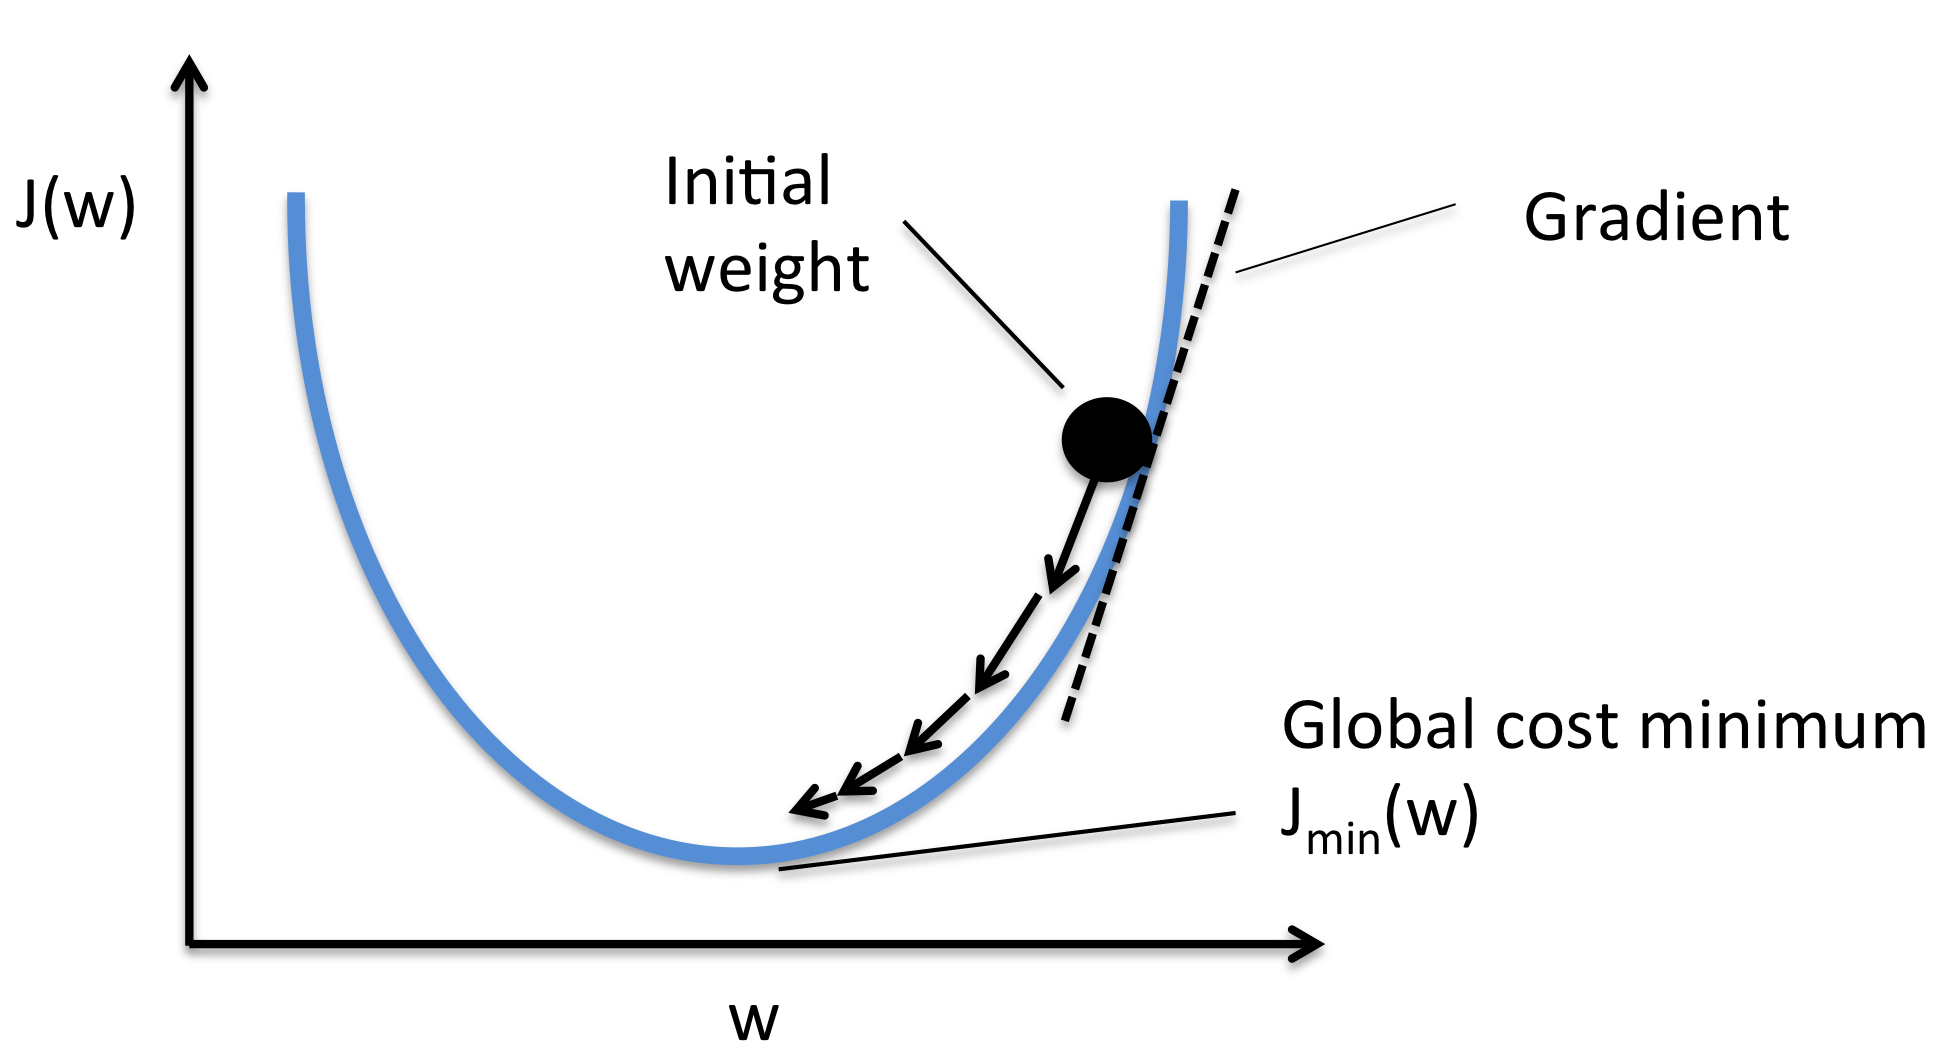
\includegraphics[width=1\columnwidth,keepaspectratio]{img/sgd.png}
	\caption{Visualisierung des Gradienten und der Loss-Funktion (J(w) = Loss; w = Parameteränderung)}
	\label{fig:sgd}
\end{figure}
\subsubsection{Perceptron}
Der Perceptron-Algorithmus basiert auf dem SGDClassifier.
Hinter der Perceptron-Implementierung steckt lediglich ein SGDClassifier mit spezieller Konfiguration.\\
Die Perceptron-Implementierung benutzt in der Konfiguration die Loss-Funktion \glqq perceptron\grqq{}, keine Strafe bei falscher Klassifizierung und eine konstante Lernrate.
\subsubsection{AdaBoostClassifier}
AdaBoost gehört zu der Familie der Ensemble-Learner.
Ensemble-Learning ist ein Zusammenschluss von mehreren unterschiedlichen Klassifizieren, welche mit einem Voting-Verfahren eine schlussendliche Klassifizierung durchführen.
Ensemble-Learning verfolgt die Annahme, dass mehrere Algorithmen im Plenum eine bessere Aussage abliefern können, als einen Algorithmus alleine.
Bei vielen Ensemble-Verfahren werden alle Klassifizierer parallel trainiert und geben ihr Votum gleichzeitig ab.\\
Adaboost verwendet jedoch die Methode des \glqq Boosting\grqq{}, welche Ähnlichkeit mit der Theorie der genetischen Algorithmen hat.
Bei Adaboost wird ein Algorithmus trainiert, validiert und als Ursprung verwendet. Alle zusätzlichen Algorithmen, welche das finale Voting durchführen, werden vom Ursprungsalgorithmus abgeleitet.
Es werden jedoch bei den Abkömmlingen die internen Parameter schrittweise verbessert und versucht die Fehler des \glqq Vater-Algorithmus\grqq{} zu vermeiden.
AdaBoost kann verbessert werden, indem die Anzahl von Vererbungsschritten angepasst wird.
\subsubsection{RandomForestClassifier}
RandomForest gehört ebenfalls zur Familie der Ensemble-Learner.
RandomForest, wie der Name schon sagt, ist eine Zusammensetzung von einer Vielzahl von unterschiedlichen DecisionTrees.\\
DecisionTree ist ebenfalls ein Algorithmus, der für die Klassifizierung verwendet werden kann.
Der DecisionTree-Algorithmus baut schrittweise eine Baumstruktur von Entscheidungszweige auf, um eine Klassifizierungsaufgabe zu meistern. 
DecisionTrees können verbessert werden, indem die Tiefe der Äste oder die Anzahl der Äste angepasst werden kann.
Bei stetiger Erhöhung der Tiefe oder der Anzahl der Äste, steigt auch die Zeitkomplexität der DecisionTrees.\\
RandomForest verwendet nun eine Vielzahl von DecisionTrees, die alle unterschiedliche Tiefen oder Anzahl Äste besitzen.
Dadurch können Entscheidungsausreisser aufgefangen und durch den Mehrheitsentscheid gedämpft werden.\\
RandomForests können oft eine sehr hohen Score bei der Precision erzielen.
\subsection{Klassifizierung mittels Machine-Learning}
\subsubsection{Konfiguration}
\subsubsection{}
\subsection{Evaluierung}
Da es sich in diesem Experiment um eine binäre Klassifizierung handelt, werden Metriken wie F1-Score, Precision und Recall verwendet.
Dazu müssen zuerst die folgenden Klassifizierungskategorien erläutert werden:
\begin{itemize}
	\item Richtig Positiv: Die Webpage wurde als Menüseite klassifiziert und ist eine Menüseite
	\item Falsch Positiv: Die Webpage wurde als Menüseite klassifiziert, ist aber keine Menüseite
	\item Falsch Negativ: Die Webpage wurde nicht als Menüseite klassifiziert, ist aber eine Menüseite
	\item Richtig Negativ: Die Webpage wurde nicht als Menüseite klassifiziert und ist keine Menüseite
\end{itemize}
Jede klassifizierte Webpage lässt sich in eine dieser Kategorie einordnen.
Anhand dieser Kategorien lässt sich für den gesamten Datensatz die oben genannten Metriken berechnen:\\
\[Precision=\frac{\text{Richtig Positiv}}{\text{Richtig Positiv} + \text{Falsch Positiv}}\]\\
Die Precision definiert das Verhältnis der korrekt positiv klassifizierten Menüseiten zu allen durch den Algorithmus als positiv klassifizierten Menüseiten.\\
\[Recall=\frac{\text{Richtig Positiv}}{\text{Richtig Positiv} + \text{Falsch Negativ}}\]\\
Der Recall definiert das Verhältnis der korrekt positiv klassifizierten Proben zu allen tatsächlichen Menüseiten.\\
\[F_{1}=\frac{\text{Precision} \times \text{Recall}}{\text{Precision} + \text{Recall}}\]\\
Anhand des F1-Scores wird die Genauigkeit der Klassifizierung gemessen.
Für jede Methode und jede Konfiguration der Klassifizierung werden diese Scores berechnet, um eine Aussage machen zu können, wie gut sie sind.
\section{Webapplikation}
\subsection{Beschreibung der Technologie}
\subsection{Beschreibung der Architektur}
\subsection{Search Engine}
\subsubsection{Beschreibung der Technologie}
\subsubsection{Konfiguration}
\newpage

\chapter{Vorgehen}
\section{Webcrawler}
\subsection{Erarbeitung des Seeds}
Als Quelle für das Abrufen von Websites dient das Seed.
Das Ziel war es, dieses mit möglichst vielen URLs von Schweizer Restaurant-Websites zu füllen.
Dafür wurden zwei Ansätze verfolgt.
Ein Verein Schweizer Restaurants, namentlich Lunch-Check\footnote{\url{https://www.lunch-check.ch/}} wurde angefragt, ob sie eine Liste ihrer Mitglieder zur Verfügung stellen.
Zudem wurde der OpenStreetmap-API\footnote{\url{https://www.openstreetmap.ch/}} genutzt, um die darin enthaltenen Restaurant-URLs abzufragen.
Die Daten aus beiden Quellen wurden zusammengeführt und dienen nun als Seed für die Abfragen des Webcrawlers.
\subsection{Erarbeitung des Webcrawlers}
Als erstes fand eine Einarbeitung in die Thematik von Docker statt, um StormCrawler damit zu betreiben.
Apache Storm ist ebenfalls thematisiert worden, da StormCrawler darauf basiert.
Danach folgte die Einarbeitung in StormCrawler.
Zu Beginn war das Ziel, die Standardtopologie zu verstehen.
Sobald die Standardtopologie funktionierte, fanden Anpassungen statt, welche zur Erstellung der Rohdaten für den Gold Standard dienten.
Explizit ist die Erstellung des Bolts zu erwähnen, welcher für das Schreiben der Output-Dateien zuständig ist.
Dieser wurde zudem mit einer Sprachdetektion erweitert, welche erkennt, ob die Sprache der Webpage deutsch ist.
\subsection{Verwendete Technologien}
\subsubsection{StormCrawler}
Es fand keine Evaluation zur Findung eines geeigneten Webcrawlers statt.
Stormcrawler wird eingesetzt, da an der Hochschule für Technik und Wirtschaft Chur ein Team bereits mit diesem arbeitet und dadurch Know-how besitzt.
Dieses Team, speziell ein wissenschaftlicher Mitarbeiter, hat Support angeboten, weshalb die Entscheidung getroffen wurde, Stormcrawler zu verwenden.
\subsubsection{Docker}
Stormcrawler wurde nicht direkt installiert, sondern mittels Docker-Container aufgesetzt.
Dies aus dem Grund, dass dadurch eine Skalierung einfach möglich ist.
Zudem ist die Installation hinfällig, da auf Docker Hub\footnote{\url{https://hub.docker.com/}} bereits fertige Images von Apache Storm und StormCrawler vorhanden sind.
\section{Gold Standard}
\subsection{Crawlen der Rohdaten}
Das Crawlen der Rohdaten war mit diversen Komplikationen verbunden.
Die Performance des Webcrawlers war zu Beginn nicht zufriedenstellend, es wurden lediglich ca. 30 Webpages pro Minute gespeichert.
Trotzdem wurde ein erster Rohdatensatz mit dieser Performance gecrawlt, auf dem das erste manuelle Labeling durchgeführt wurde.
Bei diesem Rohdatensatz wurden nur die als deutsch detektierten Webpages gespeichert, somit konnte die Abdeckung des Seeds nicht ausgewertet werden.
Der Crawler wurde nochmals angepasst, sodass alle Webpages gespeichert werden, dies ermöglicht eine genauere Analyse der Rohdaten.
Die Spracherkennung wurde zudem so angepasst, dass die Anzahl zu erkennender Sprachen eingeschränkt wurden und die Sprachdetektion nicht für jede Webpage neu gestartet wurde, was eine massive Performancesteigerung zur Folge hatte.
Diverse weitere Crawldurchläufe wurden gemacht und die gecrawlten Daten analysiert.
Diese Analysen haben ergeben, dass einzelne Websites aus dem Seed enorm viele Webpages beinhalten, zum Teil über 30'000.
Diese URLs dieser Websites wurden aus dem Seed entfernt, da sie keine typischen Restaurant-Webseiten repräsentieren.
Für die zweite Durchführung des manuellen Labelings wurden die Rohdaten mit dem angepassten Seed neu gecrawlt.
%- Auführen der Crawl-Analyse
\subsubsection{Erarbeitung des Entscheidungsrasters}
Das Entscheidungsraster ist die Grundlage des manuellen Labeling der Rohdaten.
Für dieses wurden die folgenden Entscheidungen getroffen:
\begin{itemize}
	\item Die Webpage muss auf Deutsch verfasst sein
	\item Der Anbieter muss entweder ein Restaurant, Take-Away oder Lieferdienst sein
	\item Der Text muss statisch im HTML vorhanden sein, da dynamisch gerenderte Informationen vom Webcrawler nicht gespeichert werden
	\item Es muss ein Menü, also eine Kombination aus mehreren Speisen oder eine einzelne Speise vorhanden sein
	\item Eine genauere Beschreibung oder der Preis muss vorhanden sein
	\item Getränkekarten werden explizit als negativ gelabelt
\end{itemize}
Bei der Klassifizierung wird zudem unterschieden, ob es sich um ein zeitlich begrenztes Angebot handelt, da diese Angebote zu einem späteren Zeitpunkt eventuell zusätzlich erkannt werden möchten.
\subsubsection{Manuelles Labeling der Daten}
In einer ersten Durchführung des manuellen Labelings wurden ca. 1500 Dateien klassifiziert, welche das Schlüsselwort \glqq Menu\grqq{} in der URL enthalten.
Die mit dieser Heuristik gefilterten Daten entsprechen jedoch nicht einer repräsentativen Teilmenge der gesamten Rohdaten.
Darum wurde in einer zweiten Durchführung zufällig Proben aus den Rohdaten ausgewählt und manuell gelabelt.
Dadurch konnte sichergestellt werden, dass das Verhältnis von Menüseiten zu den restlichen Webpages gleich bleibt.
\subsection{Verwendete Technologien}
\subsubsection{Labeling-Tool}
Um das manuelle Labeling effizienter zu gestalten, ist ein Tool\footnote{\url{https://github.com/s-santoro/testdata_tool}} erstellt worden, welches das Labeling vereinfacht.
Dieses Tool ruft eine Webpage der zufällig extrahierten Webpages aus den Rohdaten auf und zeigt sowohl den Text, als auch den HTML-Inhalt.
Der Anwender des Tools muss anhand dieser Informationen entscheiden, ob es sich um eine Webpage mit Menüinformationen handelt und ob diese zeitlich begrenzt sind.
Mittels Shortkeys findet die Klassifizierung statt.
Das Tool verschiebt die Datei in den entsprechenden Ordner und zeigt die Informationen der nächsten Webpage an.
\section{Klassifikation}
\subsection{Preprocessing}
Die Basisfunktionen des Preprocessings orientieren sich an einem Online-Artikel von Usman Malik\footnote{\url{https://stackabuse.com/text-classification-with-python-and-scikit-learn/}}.
Teile der darin beschriebenen Funktionen wurden angepasst und übernommen.
Weiter wurde erkannt, dass Preise mittels Regulären Ausdrücken erkannt werden müssen, damit diese Informationen nicht verloren gehen.
Darum ist eine Methode entwickelt worden, die diese Aufgabe erledigt.
Für die Funktion der Stammformreduktion ist nach einer entsprechenden Funktion gesucht worden, welche diese Aufgabe für die deutsche Sprache verrichtet.
Über die Dokumentation des Toolkits NLTK\footnote{\url{https://www.nltk.org/api/nltk.stem.html}} ist Cistem, ein Stemmer für die deutsche Sprache, gefunden und später als Preprocessing-Methode implementiert worden.
Zudem ist eine deutsche Stoppwortliste aus mehreren Quellen zusammengesetzt worden.
\subsection{Regelbasierte Klassifikation}
Die erstellten Regeln sind grösstenteils anhand Beobachtungen beim manuellen Labeln entstanden.
Dabei wurde erkannt, dass Preise sowie Speisenamen und Zutaten ein markantes Merkmal von Menüseiten sind.
Diese Informationen eignen sich für eine Whitelist.
Im Gegensatz gibt es viele Websites mit Webpages wie \glqq Imperessum\grqq{}, \glqq Anfahrt\grqq{} etc. welche typische Schlagwörter beinhalten, die in einer Blacklist aufgeführt werden können.
Durch die Regel \glqq Bag of Words\grqq{} wurde derselbe Ansatz wie beim Listing verfolgt, jedoch mit dem Ziel, durch die gleichnamige statistische Methode diese Listen dynamisch zu erzeugen.
Lediglich die Regel zur Erkennung des Schlagworts \glqq menü\grqq{} ist unter der Annahme entstanden, dass Webpages eine korrekte Angabe von Informationen im Metatag \glqq Title\grqq{} verwenden.
\subsubsection{Erstellen der Konfigurationen}
Die Konfiguration wurde erstellt, um einzelne Methoden des Preprocessings sowie die Art der Klassifizierung angeben zu können.
Wo möglich wurden Schwellwerte eingebaut, um die Klassifizierung eines Dokuments regulieren zu können.
Diese Schwellwerte wurden über mehrere Iterationen verändert, um möglichst hohe Scores zu erreichen.
Die Parameter dazu sind in \cref{cap:exp_class} ersichtlich.
\subsection{Machine-Learning Klassifikation}
\subsubsection{Einleitung}
Für die Klassifizierung mit Machine-Learning wurden mehrere Algorithmen jeweils mit den Metriken F1-Score, Recall und Precision ausgewertet.
Wegen des \glqq No free lunch\grqq{}-Theorems wurden insgesamt 14 unterschiedliche Algorithmen aus zwei unterschiedlichen Online-Artikeln zusammengetragen und stetig anhand ihrer Metriken verglichen.
Alle Algorithmen wurden jeweils mit ihrer Standardkonfiguration trainiert und anschliessend validiert, um einen möglichst unverzerrten Vergleich zu haben.
Schrittweise wurden folgende Pipelinekomponenten angepasst und versucht, einen optimalen Wert zu ermitteln.
\begin{enumerate}
	\item Dimensionsreduktion der Features 
	\item Angabe von Klassenverteilung
	\item Anwendung von N-Gramme (N={1,2,3})
	\item Anwendung von einfachen Preprocessingschritten
	\item Anwendung von fortgeschrittenen Preprocessingschritten
	\item Anzahl extrahierter Features
\end{enumerate}
Ebenfalls wurde für die Feature-Extraction die Methoden Bag-of-Words mit Worthäufigkeit, TF-IDF und zu einem späteren Zeitpunkt noch Bag-of-Words ohne Worthäufigkeit verwendet.
\subsubsection{Dimensionsreduktion der Features}
Bei der Dimensionsreduktion der Features wurde mittels LSA (Latent Sentiment Analysis)\footnote{\url{https://scikit-learn.org/stable/modules/decomposition.html}} versucht, aus einer Vielzahl von Features nur die Aussagekräftigsten zu ermitteln.
Dies wird erreicht, indem SLA Beziehungen von Wörtern mit ähnlicher Bedeutung erkennt.
Es wurde für alle drei Feature-Extraction Methoden keine Begrenzung der Anzahl Features vorgenommen und erst mit LSA beziehungsweise der direkten Scikit-Learn Implementierung "TruncatedSVD" die Feature-Reduktion vorgenommen.
\subsubsection{Klassenverteilung}
Da die Daten aus dem Goldstandard eine sehr ungleiche Verteilung von positiven und negativen Samples aufweist, wurde die Klassengewichtung anhand dieser Verteilung berechnet.
Die Gewichtung, auf ein positives Sample folgen 10.32 negative Samples, wurde den Algorithmen fürs Trainieren mitgegeben.
Die Gewichtung konnte nicht allen Algorithmen zugewiesen werden, da manche während dem Training solche Informationen nicht verwerten können.
\subsubsection{N-Gramme}
Die verwendeten Feature-Extraction Methoden bieten die Möglichkeit N-Gramme als Features zu extrahieren.
Aufgrund von verschiedenen Visualisierungen der Textdaten wurde erkannt, dass es Sinn macht, die Verwendung von Bi- und Trigrammen zu prüfen.
Die Scikit-Learn Extrahierungsmethoden bieten einfache Schnittstelle für die Extrahierung von N-Grammen.
\subsubsection{Einfaches Preprocessing}
\subsubsection{Fortgeschrittenes Preprocessing}

\subsubsection{Erstellen der Konfigurationen}
\section{Produktive Pipeline}
\section{Webapplikation}
\subsection{Erarbeitung der Webapplikation}
\subsection{Verwendete Technologien}
\subsubsection{Frontend-Komponenten}
\subsubsection{Backend-Komponenten}
\subsection{Search Engine}
\subsubsection{Vorgehen}
\subsubsection{Verwendete Technologien}
\newpage

\chapter{Benutzung der Webapplikation}

\newpage


\chapter{Fazit}
In diesem Teil werden Erkennisse der jeweiligen Bereiche aufgeführt.
Diese wurden während der Arbeit erkannt und als wichtig angesehen.
\section{Webcrawler}
Eine Evaluation des Webcrawlers wäre von Vorteil gewesen.
StormCrawler hat zwar die Funktion erfüllt, dieser ist jedoch dafür ausgelegt, eine enorme Masse an Websites und Webpages zu crawlen.
Dies ist jedoch keine Hauptanforderung in dieser Arbeit gewesen.
Dafür wäre ein Webcrawler, welcher auch dynamisch generierte Websites handhaben kann, von Vorteil gewesen.
\section{Klassifizierung}
Für die Klassifizierung hätte eine Preprocessing-Methode zur Erkennung des Hauptinhalts einer Webpage einen grossen Benefit bewirkt.
Beim manuellen Labeling wurde erkannt, dass viele Webpages nicht relevante oder sogar irreführende Informationen im Kopf- und Fussteil beinhalten.
Der Gold Standard sollte ein zweites Mal gelabelt werden, damit dieser nach dem Vier-Augen-Prinzip kontrolliert werden würde.
Von diesem Schritt wurde jedoch aus zeitlichen Gründen abgesehen.
Um die regelbasierte Klassifikation zu verbessern, wären komplett neue Regeln sowie das erweitern und anpassen der Listen wertvoll.
\newpage

\chapter{Selbstständigkeitserklärung}
\label{sec:erklaerung}
\vspace{0 cm}
Wir erklären hiermit, dass wir die vorliegende Arbeit selbstständig und ohne fremde Hilfe verfasst und keine anderen Hilfsmittel als angegeben verwendet haben. Insbesondere versichern wir, dass wir alle wörtlichen und sinngemässen Übernahmen aus anderen Werken als solche kenntlich gemacht haben.
\\
\\
Name: Sandro Santoro
\\	
Ort, Datum: \hspace{4cm}Unterschrift:
\\
\\
\\
Name: Gian Brunner
\\
Ort, Datum: \hspace{4cm}Unterschrift:
\\
\\





\newpage

%Literaturverzeichnis
\bibliographystyle{apacite}
\bibliography{bibfile}

%Verzeichnis aller Tabellen
\listoftables

%Verzeichnis aller Bilder
\listoffigures

\chapter{Anhang}
\section{Elektronischer Anhang}
\begin{itemize}
	\item Quelldatei OpenStreetMap für Seed (JSON-Datei)
	\item Quelldatei Lunch Check für Seed (Excel-Datei)
	\item Schlussendliches Seedfile (txt-Datei)
	\item Klassifikationsdatei (Pickle-Datei)
\end{itemize}
\section{Verlinkungen}
\subsection{Webcrawler}
\begin{itemize}
	\item Implementierung StormCrawler\\ \url{https://github.com/s-santoro/lunch-crawler/tree/master/storm-crawler-master}
	\item Angepasste Kompontenten\\
	\url{https://github.com/s-santoro/lunch-crawler/tree/master/storm-crawler-master/archetype/src/main/resources/archetype-resources/src/main/java/ntb/iks}
	\item Docker-Compose\\
	\url{https://github.com/s-santoro/lunch-crawler/tree/master/storm-cluster}
	\item Script zur Analyse der gecrawlten Rohdaten\\
	\url{https://github.com/s-santoro/lunch-crawler/blob/master/storm-crawler-master/scripts/website_histogram.py}
\end{itemize} 
\subsection{Gold Standard}
\label{app:gold_standard}
\begin{itemize}
	\item Gold Standard\\ 
	\url{https://github.com/s-santoro/lunch-crawler/blob/master/gold-standard/Gold_Standard.zip}
	\item Tool zum manuellen Labeln\\ 
	\url{https://github.com/s-santoro/lunch-crawler/tree/master/gold-standard/labeling_tool}
	\item Script zur Extrahierung zufälliger Daten aus den gecrawlten Rohdaten\\ 
	\url{https://github.com/s-santoro/lunch-crawler/blob/master/gold-standard/generate_randomfiles.sh}
\end{itemize} 
\subsection{Klassifikationspipeline}
\label{app:classification}
\begin{itemize}
	\item Datenimport\\ 
	\url{https://github.com/s-santoro/lunch-crawler/blob/master/classification/scripts/Importer.py}
	\item Preprocessing\\ 
	\url{https://github.com/s-santoro/lunch-crawler/blob/master/classification/scripts/Preprocessor.py}
	\item Regelbasierte Klassifikation\\ 
	\url{https://github.com/s-santoro/lunch-crawler/blob/master/classification/scripts/RulebasedClassifier.py}
	\item Klassifikation mittels Machine Learning\\ 
	\url{https://github.com/s-santoro/lunch-crawler/blob/master/classification/scripts/MLClassifiers.py}
	\item Evaluierung der Klassifikation\\ 
	\url{https://github.com/s-santoro/lunch-crawler/blob/master/classification/scripts/Evaluator.py}
	\item Visualisierung der Klassifikation\\ 
	\url{https://github.com/s-santoro/lunch-crawler/blob/master/classification/scripts/DataVisualizer.py}
	\item Konfiguration für regelbasierte Klassifikation\\ 
	\url{https://github.com/s-santoro/lunch-crawler/blob/master/classification/scripts/configs/ConfigurationsRB.py}
	\item Konfiguration für Klassifikation mittels Machine Learning\\ 
	\url{https://github.com/s-santoro/lunch-crawler/blob/master/classification/scripts/configs/ConfigurationsML.py}
	\item Stoppwortliste\\ 
	\url{https://github.com/s-santoro/lunch-crawler/blob/master/classification/stopwords_no_umlaute.txt}
	\item Getränkeliste\\ 
	\url{https://github.com/s-santoro/lunch-crawler/blob/master/classification/beverage_list.txt}
	\item Blacklist\\ 
	\url{https://github.com/s-santoro/lunch-crawler/blob/master/classification/blacklist.txt}
	\item Whitelist\\ 
	\url{https://github.com/s-santoro/lunch-crawler/blob/master/classification/whitelist.txt}
\end{itemize} 
\subsection{Produktive Pipeline}
\begin{itemize}
	\item Pipeline zur Klassifikation der Rohdaten\\ 
	\url{https://github.com/s-santoro/lunch-crawler/tree/master/prod-pipeline/classification}
	\item Script zur Standardisierung von Restaurantinformationen\\ 
	\url{https://github.com/s-santoro/lunch-crawler/blob/master/prod-pipeline/nodejs/standardize_data.js}
	\item Script zur Analyse von Restaurantinformationen\\ 
	\url{https://github.com/s-santoro/lunch-crawler/blob/master/prod-pipeline/nodejs/analyze_data.js}
\end{itemize} 




\end{document}
